\documentclass[aspectratio=169,xcolor=table]{beamer}
%aspcetratio >> 1610 169 149 54 43 32
%The themes:
% \usetheme[style=default]{mharvellous}
\usetheme[style=classic]{mharvellous}
%\usetheme[style=dark]{mharvellous}
%\usetheme[style=mracula]{mharvellous}
%*--------------------------------------------------
%\usepackage{helvet}
%*--------------------------------------------------
\usepackage{bibunits}
%\setbeamertemplate{bibliography item}{[\theenumiv]}
\setbeamertemplate{bibliography item}{\insertbiblabel}
\defaultbibliography{bibliography}
%\defaultbibliographystyle{IEEEtran}
%\defaultbibliographystyle{amsalpha}
\defaultbibliographystyle{abntex2-alf}
%\bibliography{bibliography}
%\usepackage[backend=biber,style=alphabetic,citestyle=authoryear]{biblatex}
% \addbibresource{bibliography.bib}
%\usepackage{natbib}
\usepackage{bibentry}
%*--------------------------------------------------
\usepackage{lipsum}
\usepackage{epigraph}
\usepackage{graphicx}
\usepackage{multirow}
%\usepackage{enumitem}
\usepackage{array}
%\usepackage{multimedia}
\usepackage{media9}
%\usepackage{pdfpc-movie}
\usepackage{circledsteps}
\usepackage{listings}
\usepackage[normalem]{ulem}
%\usepackage{Sweave}
%\usepackage{xkeyval}
%\usepackage{palatino}
%\usepackage{pgfpages}
\usepackage{float}
%*--------------------------------------------------
\usepackage[timeinterval=1]{tdclock}
%\usepackage[font=Times,timeinterval=1, timeduration=200,resetatpages=all]{tdclock}
%\usepackage[font=Times,timeinterval=10, timeduration=2.0, timedeath=0, fillcolorwarningsecond=white!60!yellow,timewarningfirst=50,timewarningsecond=80,resetatpages=2]{tdclock}
%*--------------------------------------------------
\usepackage{url}
\usepackage{tabularx,booktabs}
\usepackage{threeparttable}
\usepackage[absolute, overlay]{textpos}
%*--------------------------------------------------
\usepackage{framed, color}
\usepackage[tikz]{bclogo}
\usepackage{spot}
\setspotlightcolor{red!50}
% %\setspotlightstyle{star, fill=red!50}
% %\setspotlightstyle{star points=7}
\usepackage{color,soul}
%\usepackage{xcolor}
\usepackage{tcolorbox}
\usepackage{xcolor}
\usepackage[export]{adjustbox}
\usepackage{verbatim}
\usetikzlibrary{trees,shapes,arrows}
\usepackage{fancyvrb}
\usepackage{float}
%*--------------------------------------------------
\usepackage{amsmath}
\usepackage{xfrac}
\usepackage{units}
\usepackage{ulem}
\usepackage{amsmath,amssymb}
\usepackage{caption}
\usepackage{siunitx}
\usepackage{mathtools}
%*-------------------------------------------------------------------------------
%\newcolumntype{C}[1]{>{\centering\arraybackslash}m{#1}}
\newcolumntype{L}[1]{>{\raggedright\let\newline\\\arraybackslash\hspace{0pt}}m{#1}}
\newcolumntype{C}[1]{>{\centering\let\newline\\\arraybackslash\hspace{0pt}}m{#1}}
\newcolumntype{R}[1]{>{\raggedleft\let\newline\\\arraybackslash\hspace{0pt}}m{#1}}
%*-------------------------------------------------------------------------------
%\pgfpagesuselayout{2 on 1}[a4paper,border shrink=5mm]
%\setbeamertemplate{note page}[plain]
%\setbeameroption{show notes on second screen=bottom}
%*-------------------------------------------------------------------------------
\setbeameroption{hide notes}
%\setbeameroption{show only notes}
%\setbeameroption{show notes on second screen=right}
\setbeamertemplate{note page}{\pagecolor{yellow!5}\insertnote}
%*-------------------------------------------------------------------------------

%*-------------------------------------------------------------------------------
\title              {krk-RHA}
\subtitle           {Project Overview}
\author             {Diogo Alexandre Martins}
\email              {diogomartins.ac@gmail.com}
\advisor            {Advisor: Marco A. dos Reis}
\institute          {Robotics and Autonomous Systems, Senai Cimatec}
\date               {January 2022}
% \ulogo        		{Template/logosenaicimatecnegativo}
% \ulogof             {Template/logosenaicimatec2020}
% \ulogoo        		{Template/rosa-logo}
% \ulistelement    	{Template/bullet-white}

%*-------------------------------------------------------------------------------
\graphicspath{{Source/pictures/}}
%*-------------------------------------------------------------------------------
\totalNoSlidesDisabled % To turn off the total number of slides in the footer. Comment this if you want the total number of slides in the footer
%*-------------------------------------------------------------------------------
\begin{document}
%*----------- COVER -------------------------------------------------------------
 \begin{frame}[t,plain]
%*----------- sound--------------------------------
    \includemedia[
        %width=1ex,
        %height=1ex,
        %activate=pageopen,
        activate=onclick,
        deactivate=onclick,
        %passcontext,
        transparent,
        addresource=./Source/sounds/hip-hop.mp3,
        flashvars={
                    source=./Source/sounds/hip-hop.mp3
                    %&autoPlay=true
                    &autoRewind=true
                    &Play=2s
                    &repeat=always
                    %&Loop=true
        }
    ]
    {}{VPlayer.swf}
%*----------- start-page--------------------------
    \titlepage
    %*----------- notes-------------------------------
    \note[item]{Notes can help you to remember important information. Turn on the notes option.}
\end{frame}
%-
%*----------- SECTIONS ----------------------------------------------------------
% \begin{frame}{Introduction}
%     \begin{itemize}
%     \item Unmanned Aerial Vehicle
%     \item Application flexibility
%     \item Evolution of microprocessors
%     \item Miniaturization of electronic devices
%     \end{itemize}
% \end{frame}

\begin{frame}{Introduction}
    \begin{figure}
        \centering
        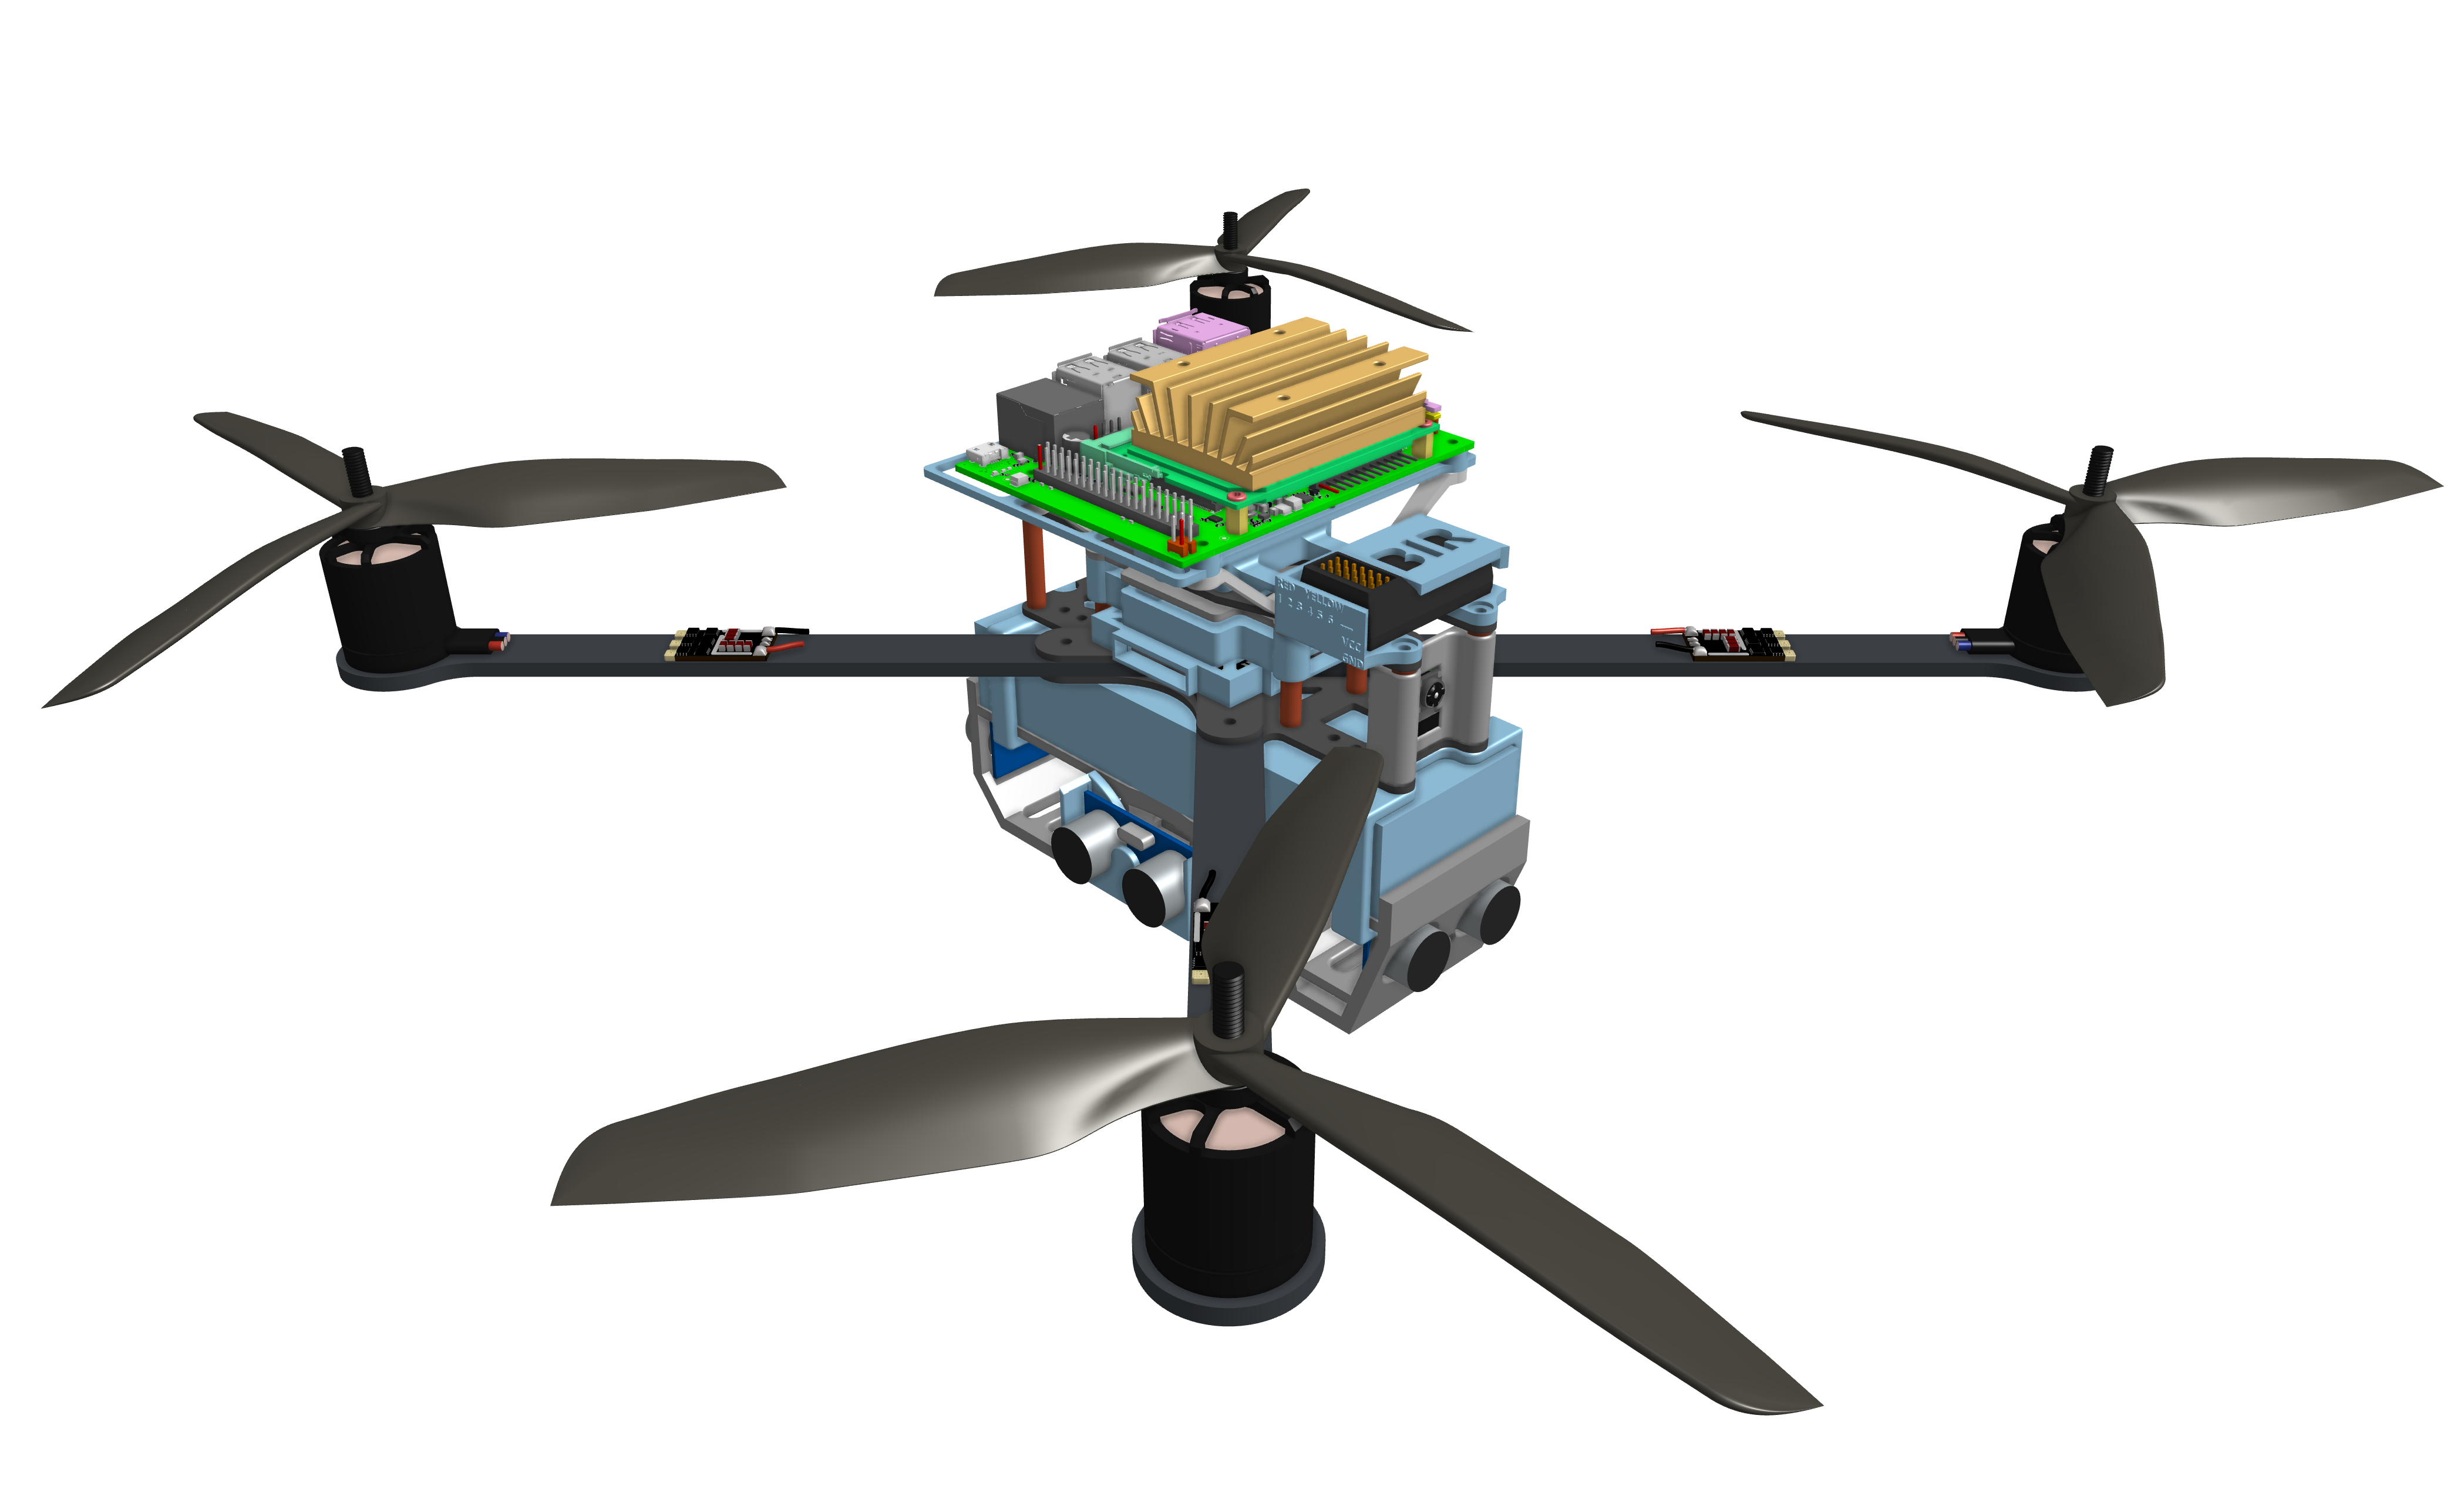
\includegraphics[width=0.8\textwidth]{img/carcara3.png}
        % \caption{Automated Inspections.}
        \label{fig:carcara}
    \end{figure}
\end{frame}

\begin{frame}{Introduction - Applications}
    \begin{columns}
        \begin{column}{0.6\textwidth}
        \begin{itemize}
            \item Mapping
            \item Transport
            \item Disaster monitoring
            \item Pesticide applications
            \item Inspection of transmission lines
            \item Infrastructure inspection
        \end{itemize}
        \end{column}
        \begin{column}{0.4\textwidth}  %%<--- here
            % \begin{center}[width=1.1\textwidth]
                \begin{figure}
                    \centering
                    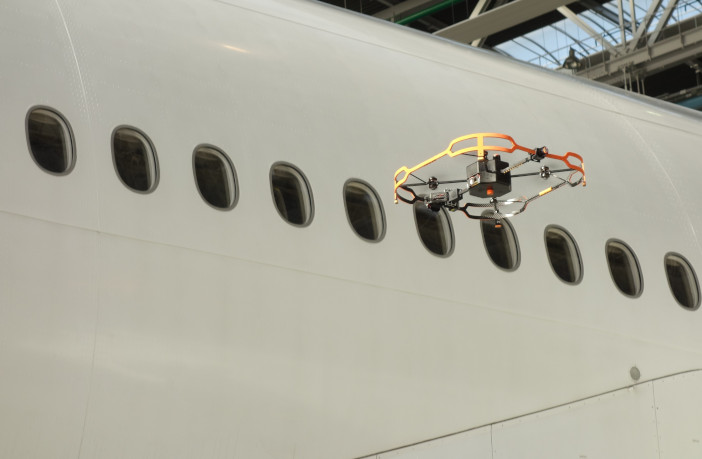
\includegraphics[width=1\textwidth]{img/inspection-drone.jpg}
                    \caption{Automated Inspections.}
                    \label{fig:uav-insp}
                \end{figure}
            %  \end{center}
        \end{column}
    \end{columns}
\end{frame}
\begin{frame}{Project Requirements}


    \begin{columns}
        \begin{column}{0.4\textwidth}
        \begin{itemize}
            \item ROS 2 framework
            \item Flight stability
            \item Real-time image processing
            \item SLAM
            \item Obstacle avoidance
            \item Autonomous navigation and landing
        \end{itemize}
        \end{column}
        \begin{column}{0.6\textwidth}  %%<--- here
            \begin{figure}
                \centering
                
\includegraphics[width=1\textwidth]{img/carcara2.png}
                \label{fig:carcara2}
            \end{figure}
        \end{column}
    \end{columns}
\end{frame}

\begin{frame}{Objective}


    \begin{columns}
        \begin{column}{0.4\textwidth}
        \begin{itemize}
            \item Build a research drone with the potential to autonomously explore unknown environments, avoid obstacles and detect areas of interest.
            % \item Autonomous landing on a fiducial mark
        \end{itemize}
        \end{column}
        \begin{column}{0.6\textwidth}  %%<--- here
            \begin{figure}
                \centering
                
\includegraphics[width=1\textwidth]{img/carcara2.png}
                \label{fig:carcara3}
            \end{figure}
        \end{column}
    \end{columns}
\end{frame}

% \begin{frame}{About the System}


% \begin{columns}
%         \begin{column}{0.4\textwidth}
%         \begin{itemize}
%             \item Underactuated system
%             \item 4 actuators, 6 degrees of freedom
%             % \item Autonomous landing on a fiducial mark
%         \end{itemize}
%         \end{column}
%         \begin{column}{0.6\textwidth}  %%<--- here
%             \begin{figure}
%                 \centering
%                 
\includegraphics[width=1\textwidth]{img/carcara2.png}
%                 \label{fig:carcara2}
%             \end{figure}
%         \end{column}
%     \end{columns}
% \end{frame}

% \begin{frame}{About the System}


% \begin{columns}
%         \begin{column}{0.4\textwidth}
%         \begin{itemize}
%             \item Underactuated system
%             \item 4 actuators, 6 degrees of freedom
%             % \item Autonomous landing on a fiducial mark
%         \end{itemize}
%         Assumptions:
%         \begin{itemize}
%             \item The quadcopter is a rigid body.
%             \item The structure is symmetric.
%             \item The center of mass of the system coincides with the origin of the coordinate system.
%         \end{itemize}
%         \end{column}
%         \begin{column}{0.6\textwidth}  %%<--- here
%             \begin{figure}
%                 \centering
%                 
\includegraphics[width=1\textwidth]{img/carcara2.png}
%                 \label{fig:carcara2}
%             \end{figure}
%         \end{column}
%     \end{columns}
% \end{frame}

% \begin{frame}{Mathematical Model}
%     \begin{itemize}
%         % \item Formulação de Newton-Euler
%         \item Rotational dynamics
%         \item 3 Degrees of freedom
%     \end{itemize}


% \begin{columns}
% \begin{column}{0.4\textwidth}
% \begin{align*}\resizebox{.6\hsize}{!}{
%         \begin{dcases}
%             &\dot{\theta} = p+ r\,cos(\phi )\,{tan}(\theta)+q\,sen(\varphi )\,{tan}({\theta})\\
%             &\dot{\phi} = q\,cos(\phi )-r\,sen(\phi )\\
%             &\dot{\psi} = \frac{r\,cos(\phi )}{cos({\theta})}+\frac{q\,sen(\phi )}{cos({\theta})}\\
%             &\dot{p} = \frac{I_{y} - I_{z}}{I_{x}}q r + \frac{\tau_{x}}{I_{x}}\\
%             &\dot{q} = \frac{I_{z} - I_{x}}{I_{y}}p r + \frac{\tau_{y}}{I_{y}}\\
%             &\dot{r} = \frac{I_{x} - I_{y}}{I_{z}}p q + \frac{\tau_{z}}{I_{z}}\\
%             &\tau_{x} = b l\, sen(\pi/4) (\Omega_{1}^{2} + \Omega_{2}^{2} - \Omega_{3}^{2} - \Omega_{4}^{2})\\
%             &\tau_{y} = b l\, sen(\pi/4) (\Omega_{1}^{2} + \Omega_{4}^{2} - \Omega_{2}^{2} - \Omega_{3}^{2})\\
%             &\tau_{z} = d (\Omega_{2}^{2} + \Omega_{4}^{2} - \Omega_{1}^{2} - \Omega_{3}^{2})
%         \end{dcases}}
%     \end{align*}
% \end{column}
% \begin{column}{0.6\textwidth}  %%<--- here
%     % \begin{center}[width=1.1\textwidth]
%      \begin{figure}
%          \centering
%          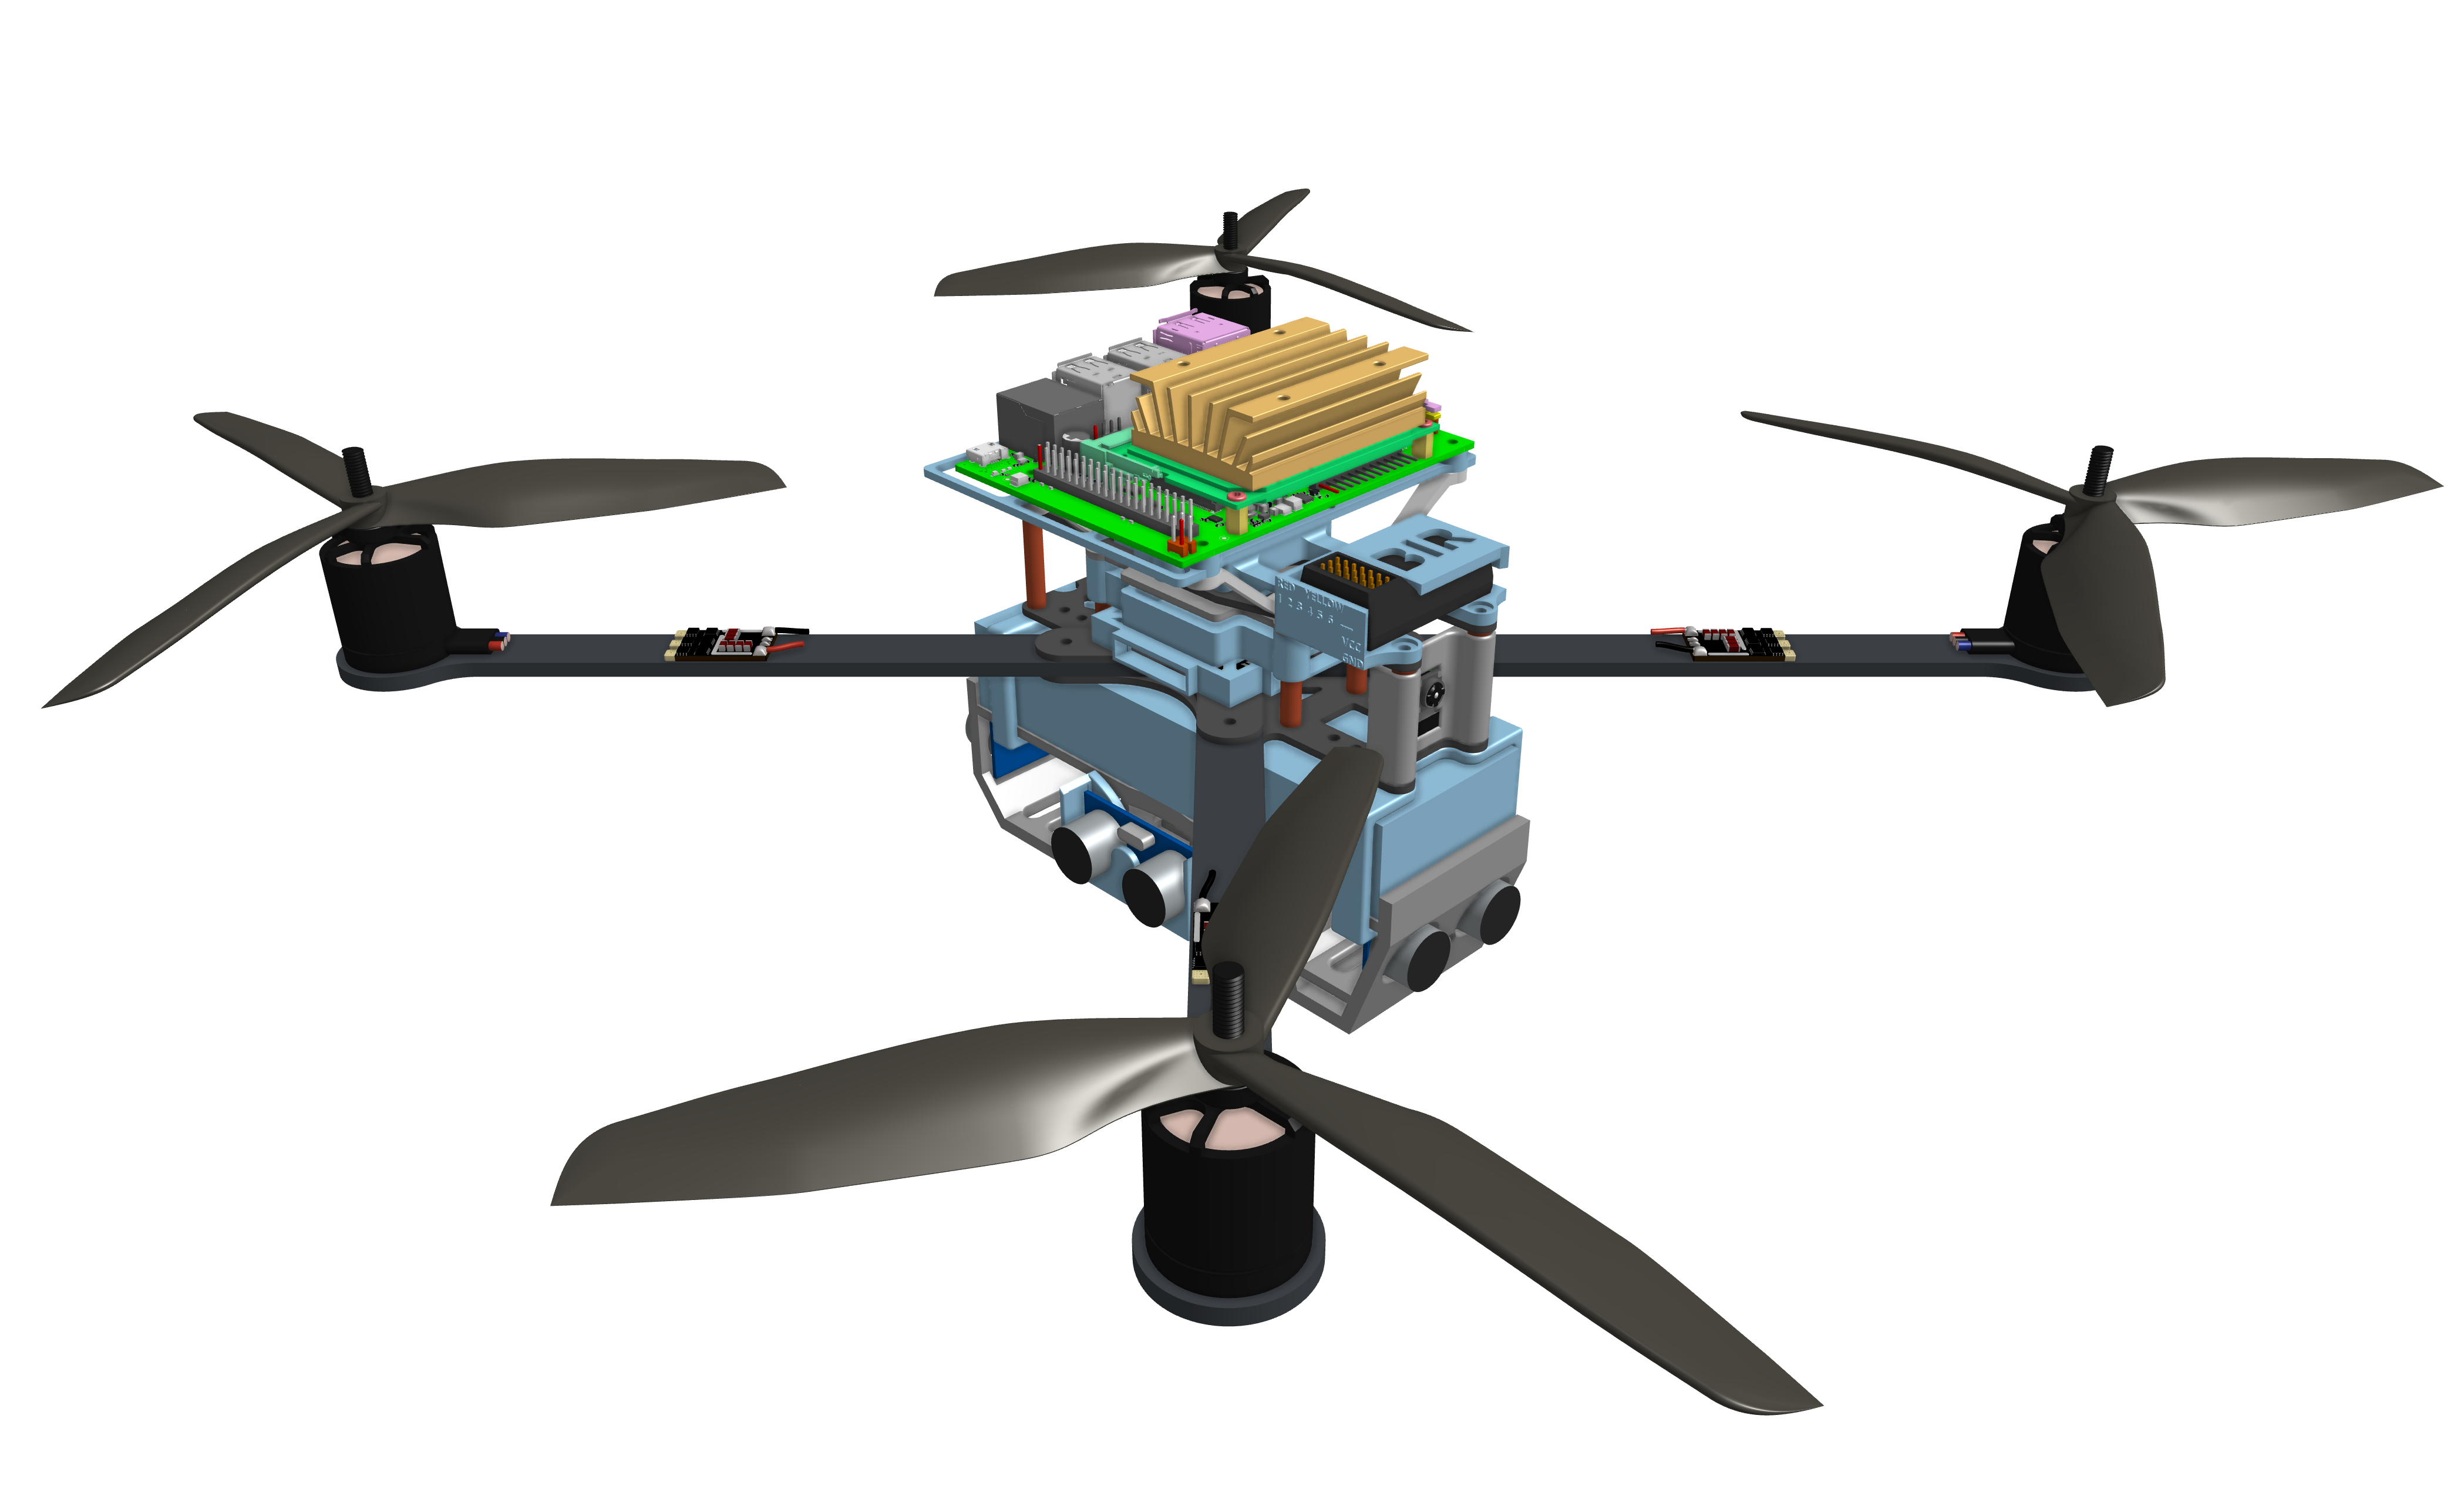
\includegraphics[width=1\textwidth]{img/carcara3.png}
%      \end{figure}
%     %  \end{center}
% \end{column}
% \end{columns}

% \end{frame}



% \begin{frame}{Mathematical Model}
%     % Sendo $\tau_{x},\tau_{y}$ e $\tau_{z}$ dados por
%     % \begin{align*}
%     % \begin{dcases}
%     %     &\tau_{x} = b l s(\pi/4) (\Omega_{1}^{2} + \Omega_{2}^{2} - \Omega_{3}^{2} - \Omega_{4}^{2})\\
%     %     &\tau_{y} = b l s(\pi/4) (\Omega_{1}^{2} + \Omega_{4}^{2} - \Omega_{2}^{2} - \Omega_{3}^{2})\\
%     %     &\tau_{z} = d (\Omega_{2}^{2} + \Omega_{4}^{2} - \Omega_{1}^{2} - \Omega_{3}^{2})
%     % \end{dcases}
%     % \end{align*}
%             \begin{itemize}
%                 \item The actuators have the same dynamics.
%                 \item The thrust factor ($b$) and drag factor($d$) are constant.
%             \end{itemize}

%     \begin{block}{Controlled Variables}
%     Angular velocities -- $p, q, r$
%     \end{block}

%     \begin{block}{Manipulated variables}
%     Rotor speeds -- $\Omega_{1},\Omega_{2},\Omega_{3},\Omega_{4}$
%     \end{block}

%     \begin{block}{Manipulated variables (prototype)}
%     PWM signals -- $PWM_{1},PWM_{2},PWM_{3},PWM_{4}$
%     \end{block}
% \end{frame}




% \begin{frame}{Technical Requirements}


%     \begin{columns}
%         \begin{column}{0.4\textwidth}
%         \begin{itemize}
%             \item ROS 2 framework
%             \item Flight stability
%             \item Real-time image processing
%             % \item Autonomous landing on a fiducial mark
%         \end{itemize}
%         \end{column}
%         \begin{column}{0.6\textwidth}  %%<--- here
%             \begin{figure}
%                 \centering
%                 
\includegraphics[width=1\textwidth]{img/carcara2.png}
%                 \label{fig:carcara2}
%             \end{figure}
%         \end{column}
%     \end{columns}
% \end{frame}


\begin{frame}{System Specification - Power}


    \begin{columns}
        \begin{column}{0.4\textwidth}
        \begin{itemize}
            % \item NVIDIA Jetson Nano
            % \item Microcontroller Teensy 4.0
            % \item MPU-9250 IMU
            \item Matek Mini Power Hub
            \item Lipo Battery 5000mAh 60C 3S
            % \item 4 x ESC Racestar 30A
            % \item 4 x Brushless Motor X2212 - 13 KV 980 II
            % \item Autonomous landing on a fiducial mark
        \end{itemize}
        \end{column}
        \begin{column}{0.6\textwidth}  %%<--- here
            \begin{figure}
                \centering
                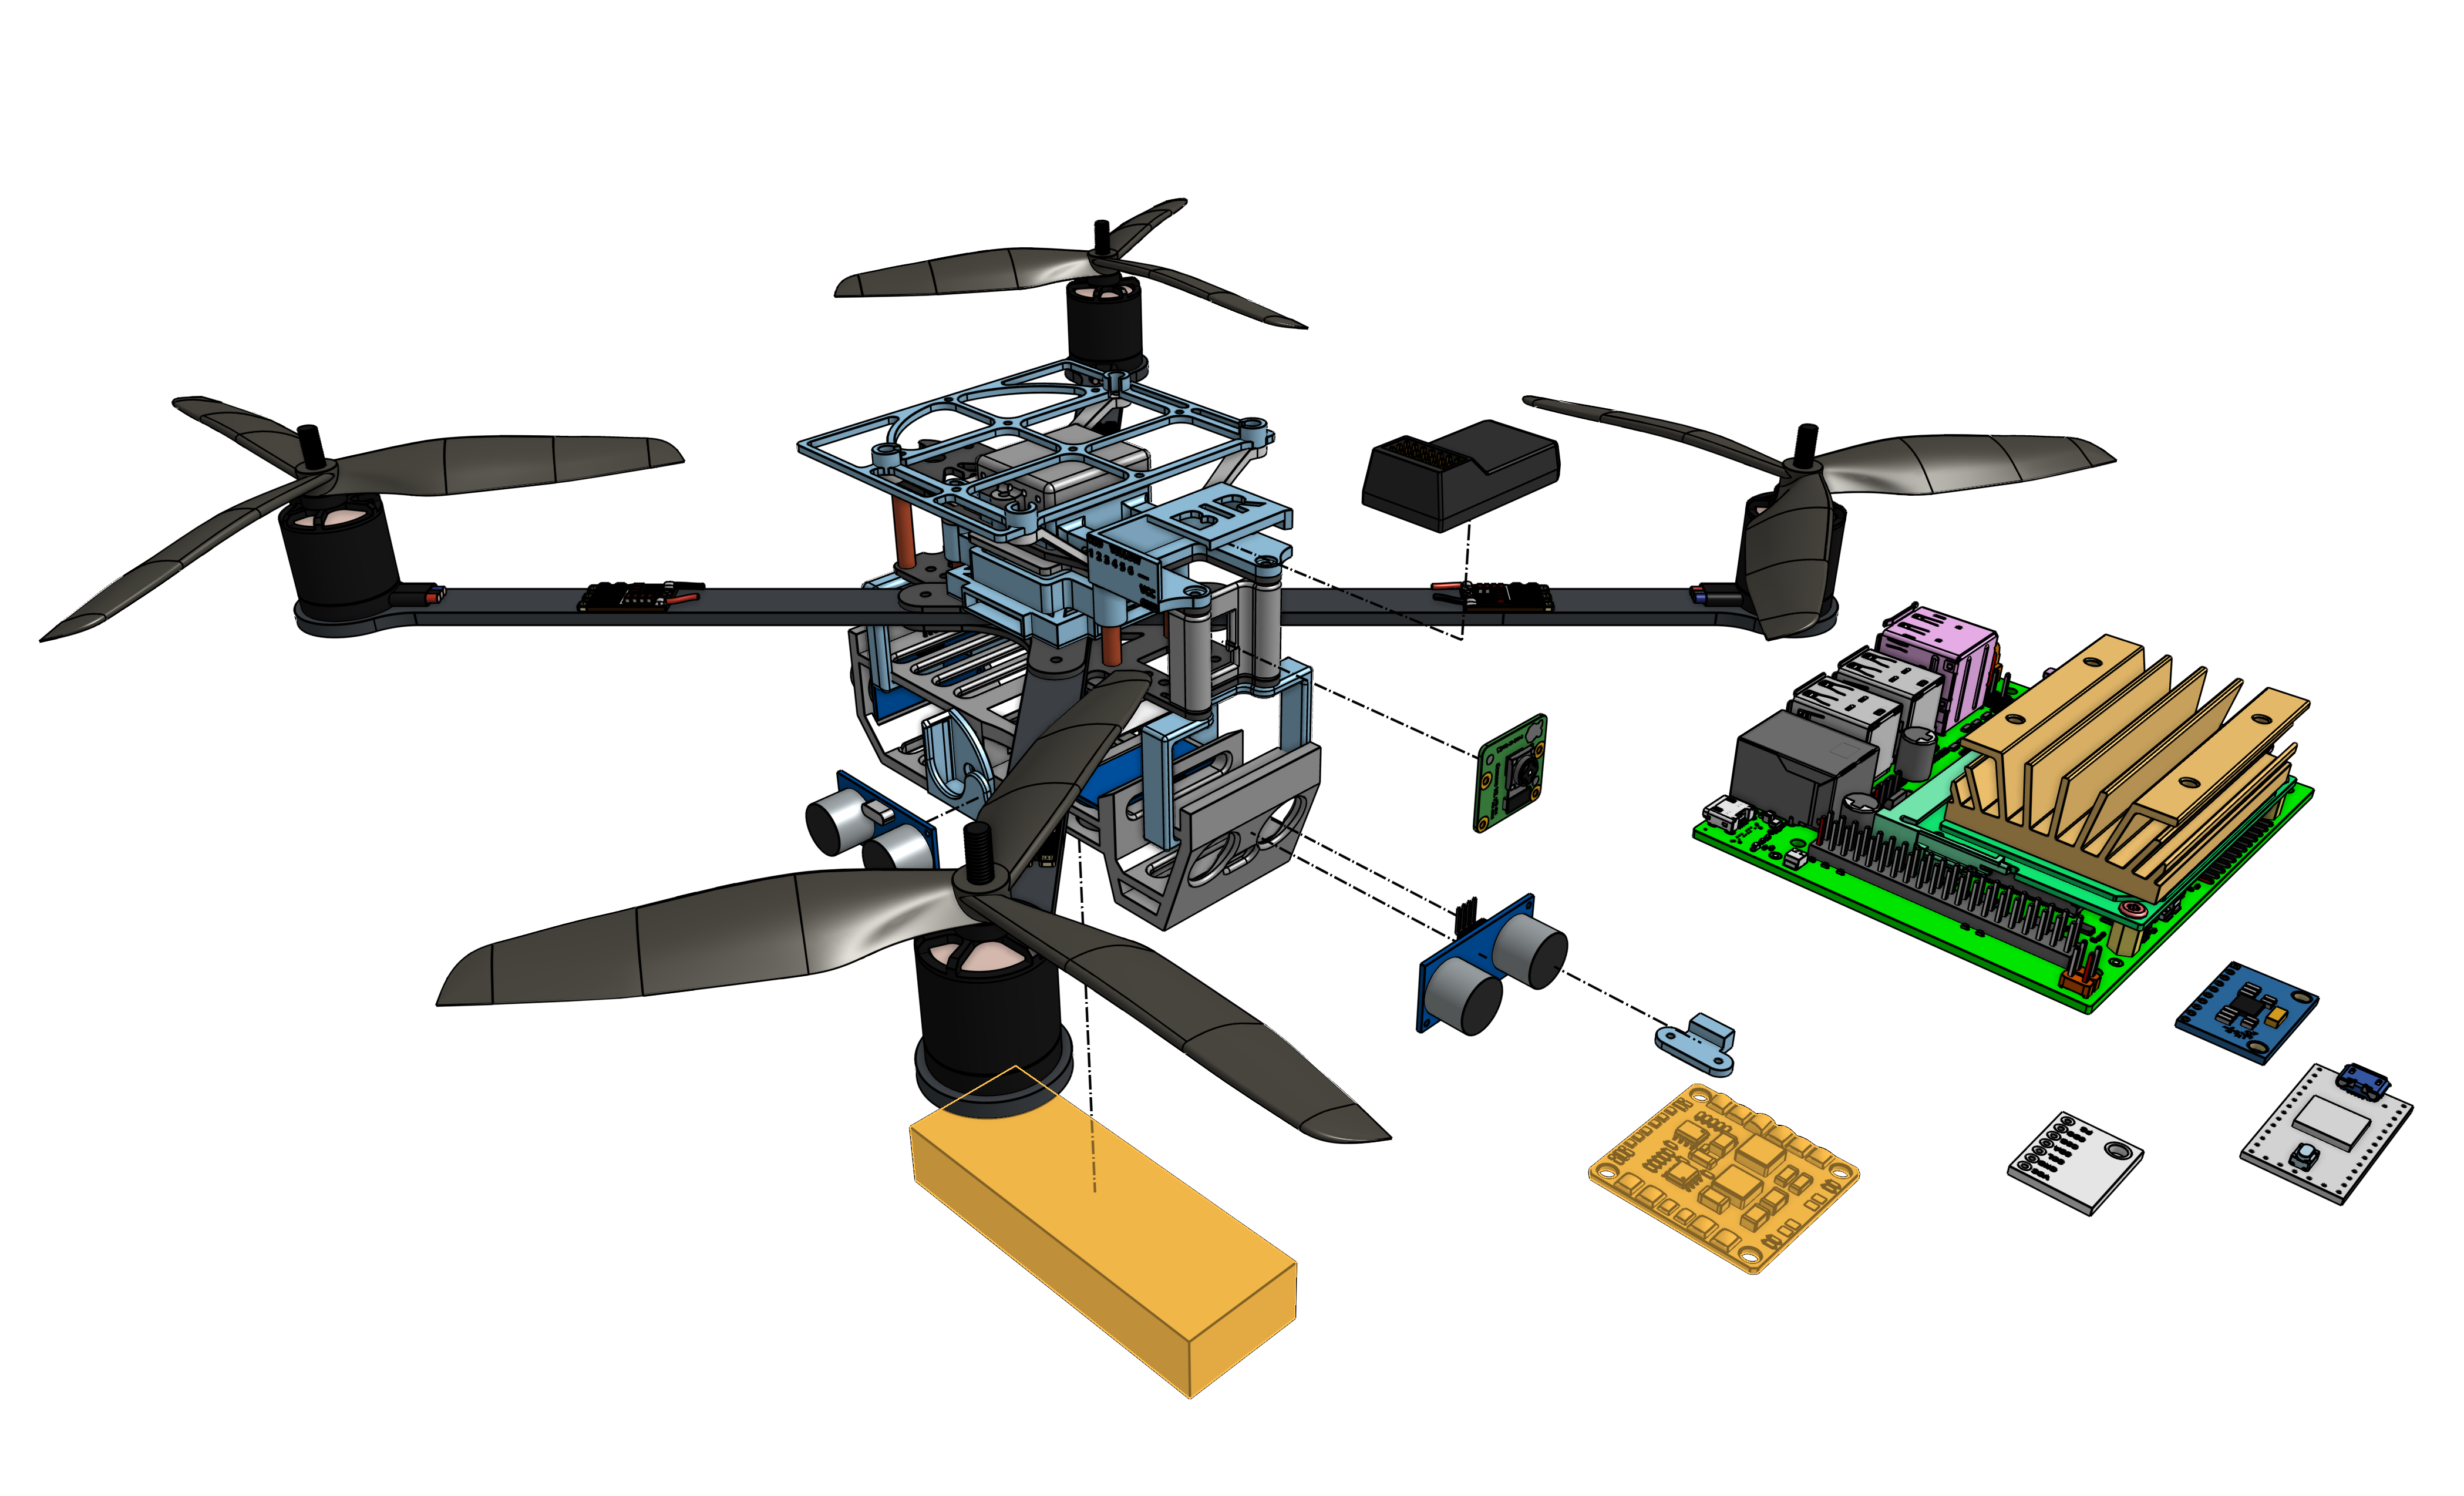
\includegraphics[width=1\textwidth]{img/exploded-power.png}
                \label{fig:power}
            \end{figure}
        \end{column}
    \end{columns}
\end{frame}

\begin{frame}{System Specification - Actuation}


    \begin{columns}
        \begin{column}{0.4\textwidth}
        \begin{itemize}
            % \item NVIDIA Jetson Nano
            % \item Microcontroller Teensy 4.0
            % \item MPU-9250 IMU
            % \item Matek Mini Power Hub
            % \item Lipo Battery 5000mAh 60C 3S
            \item 4 x ESC Racestar 30A
            \item 4 x Brushless Motor X2212 - 13 KV 980 II
        \end{itemize}
        \end{column}
        \begin{column}{0.6\textwidth}  %%<--- here
            \begin{figure}
                \centering
                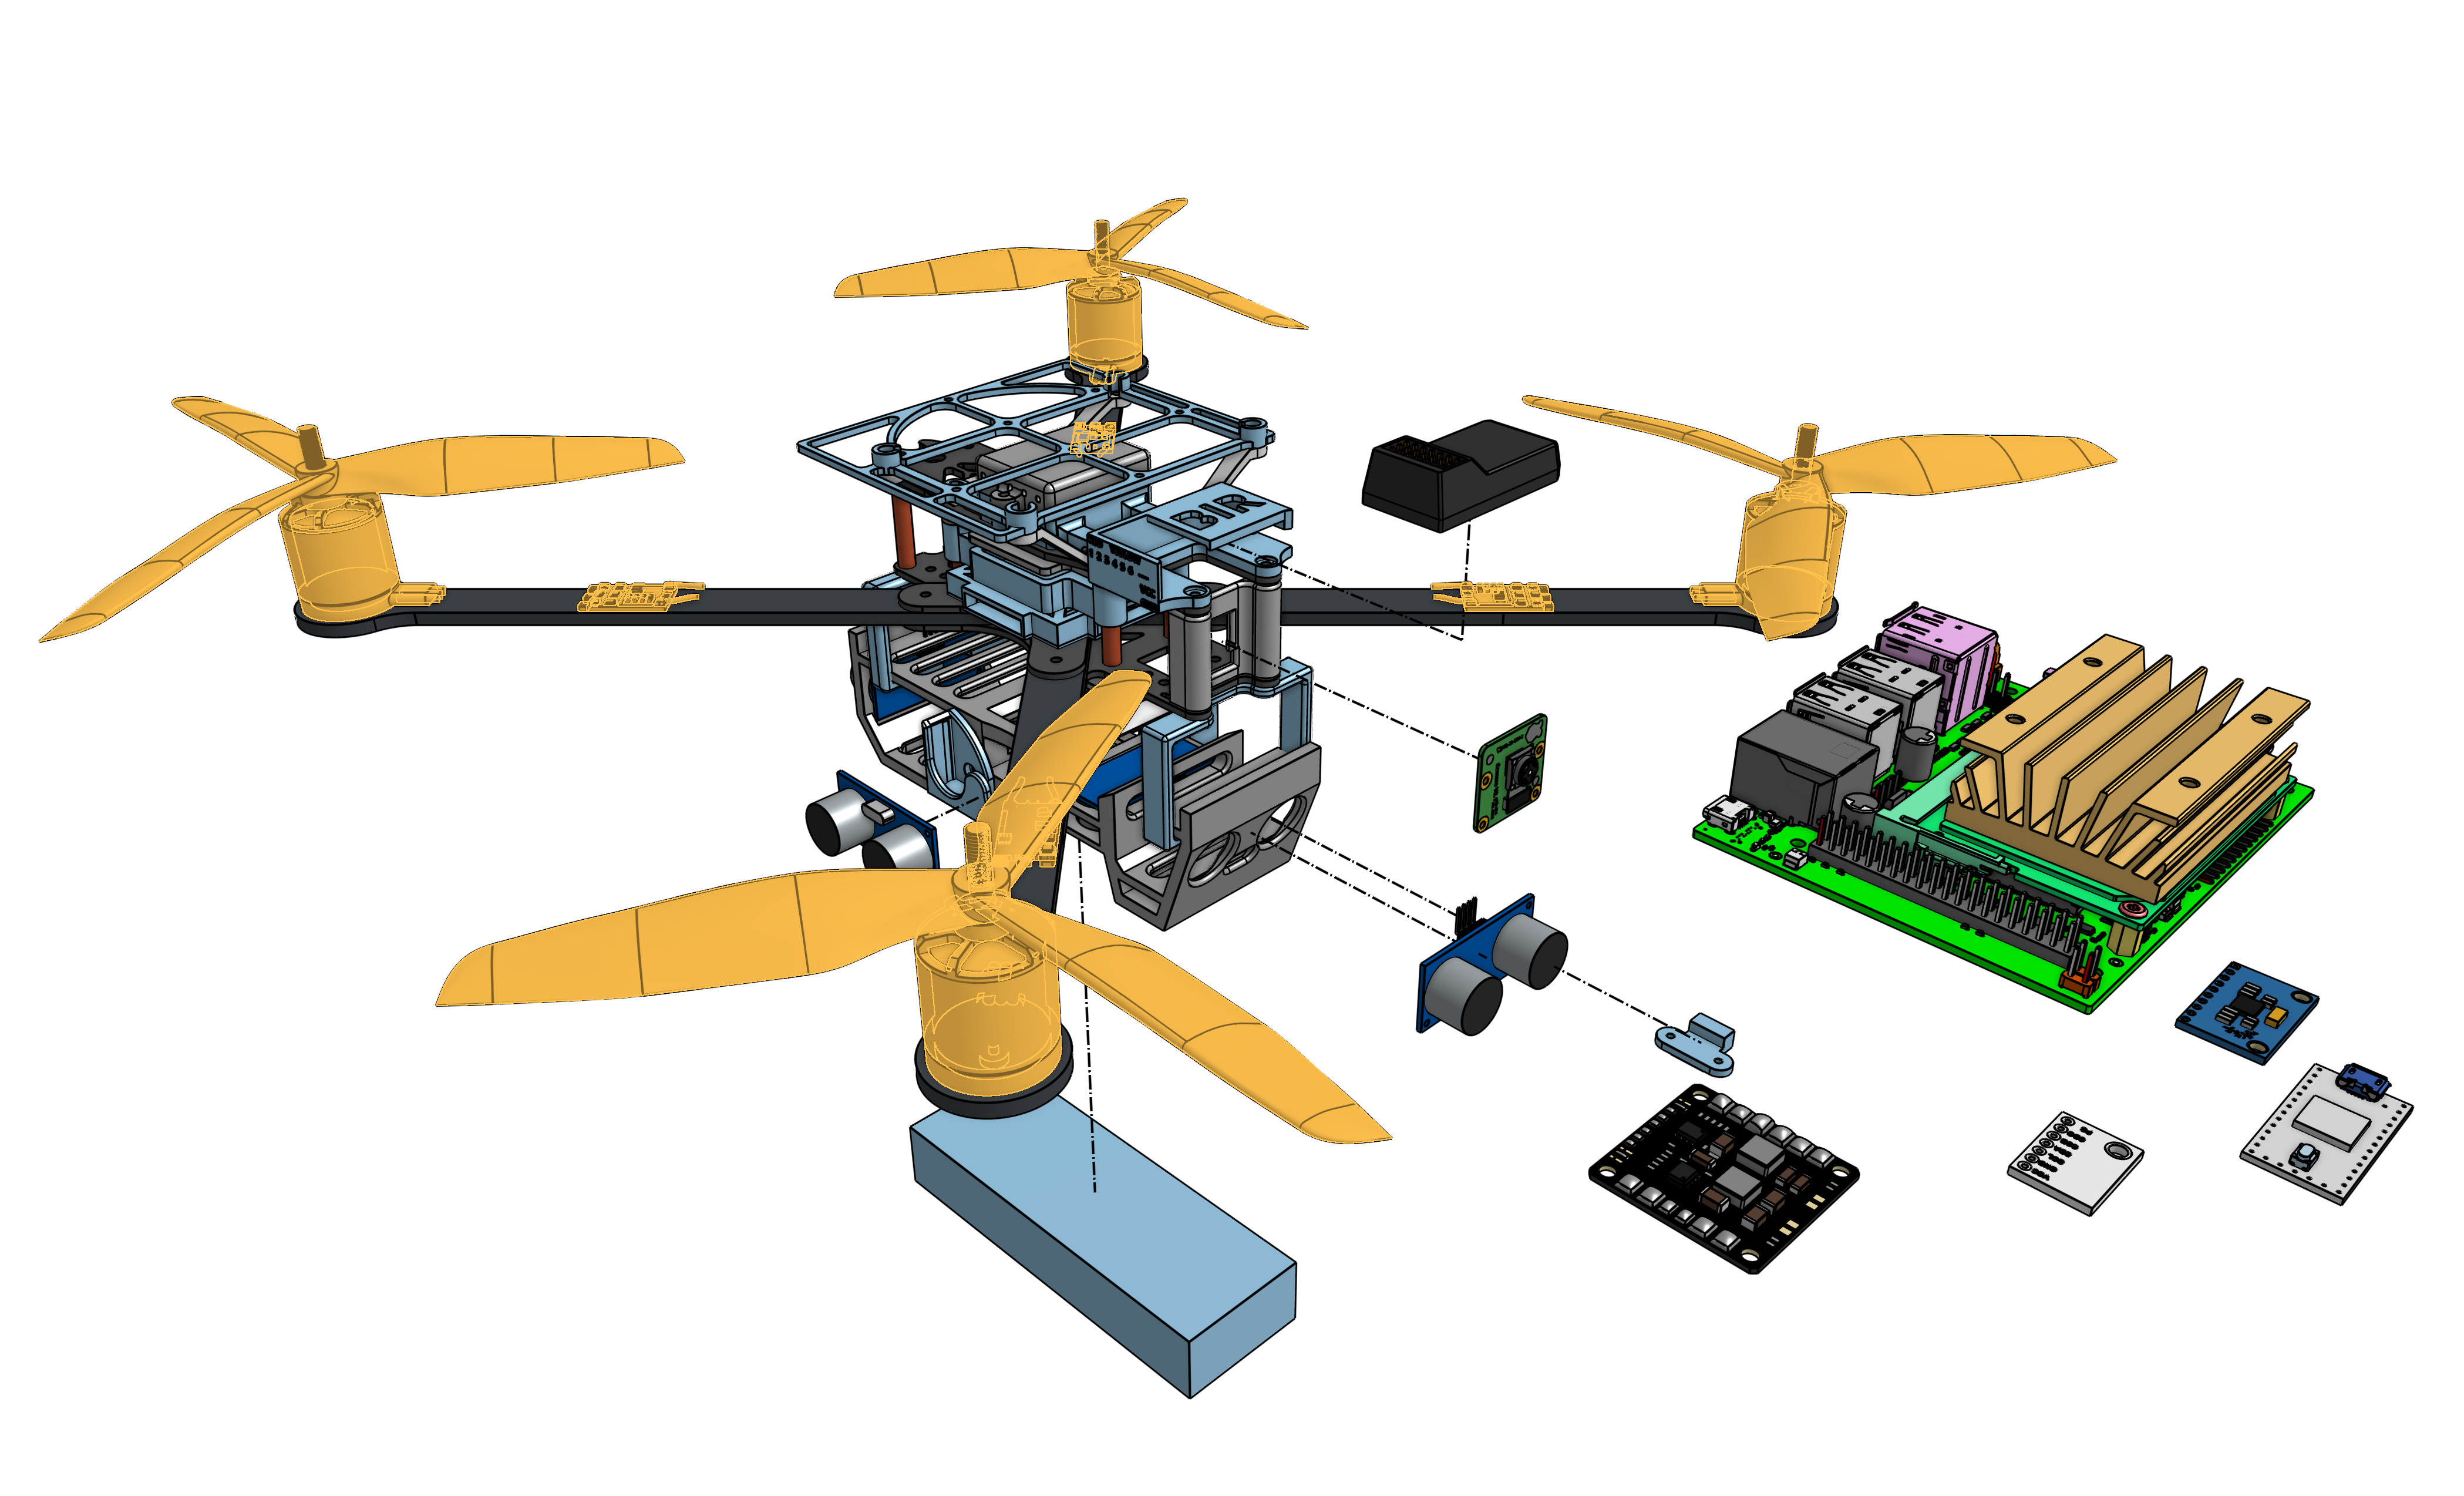
\includegraphics[width=1\textwidth]{img/exploded-actuation.png}
                \label{fig:actuation}
            \end{figure}
        \end{column}
    \end{columns}
\end{frame}

\begin{frame}{System Specification - Sensors}


    \begin{columns}
        \begin{column}{0.4\textwidth}
        \begin{itemize}
            \item IMU - MPU-9250
            \item Barometer - MS5611
            \item Laser Range Sensor - TOF10120
            \item 2 x Camera - Raspberry Pi v2 8MP (IMX219)
            \item 5 x Ultrasonic Transducer - HC-SR04
        \end{itemize}
        \end{column}
        \begin{column}{0.6\textwidth}  %%<--- here
            \begin{figure}
                \centering
                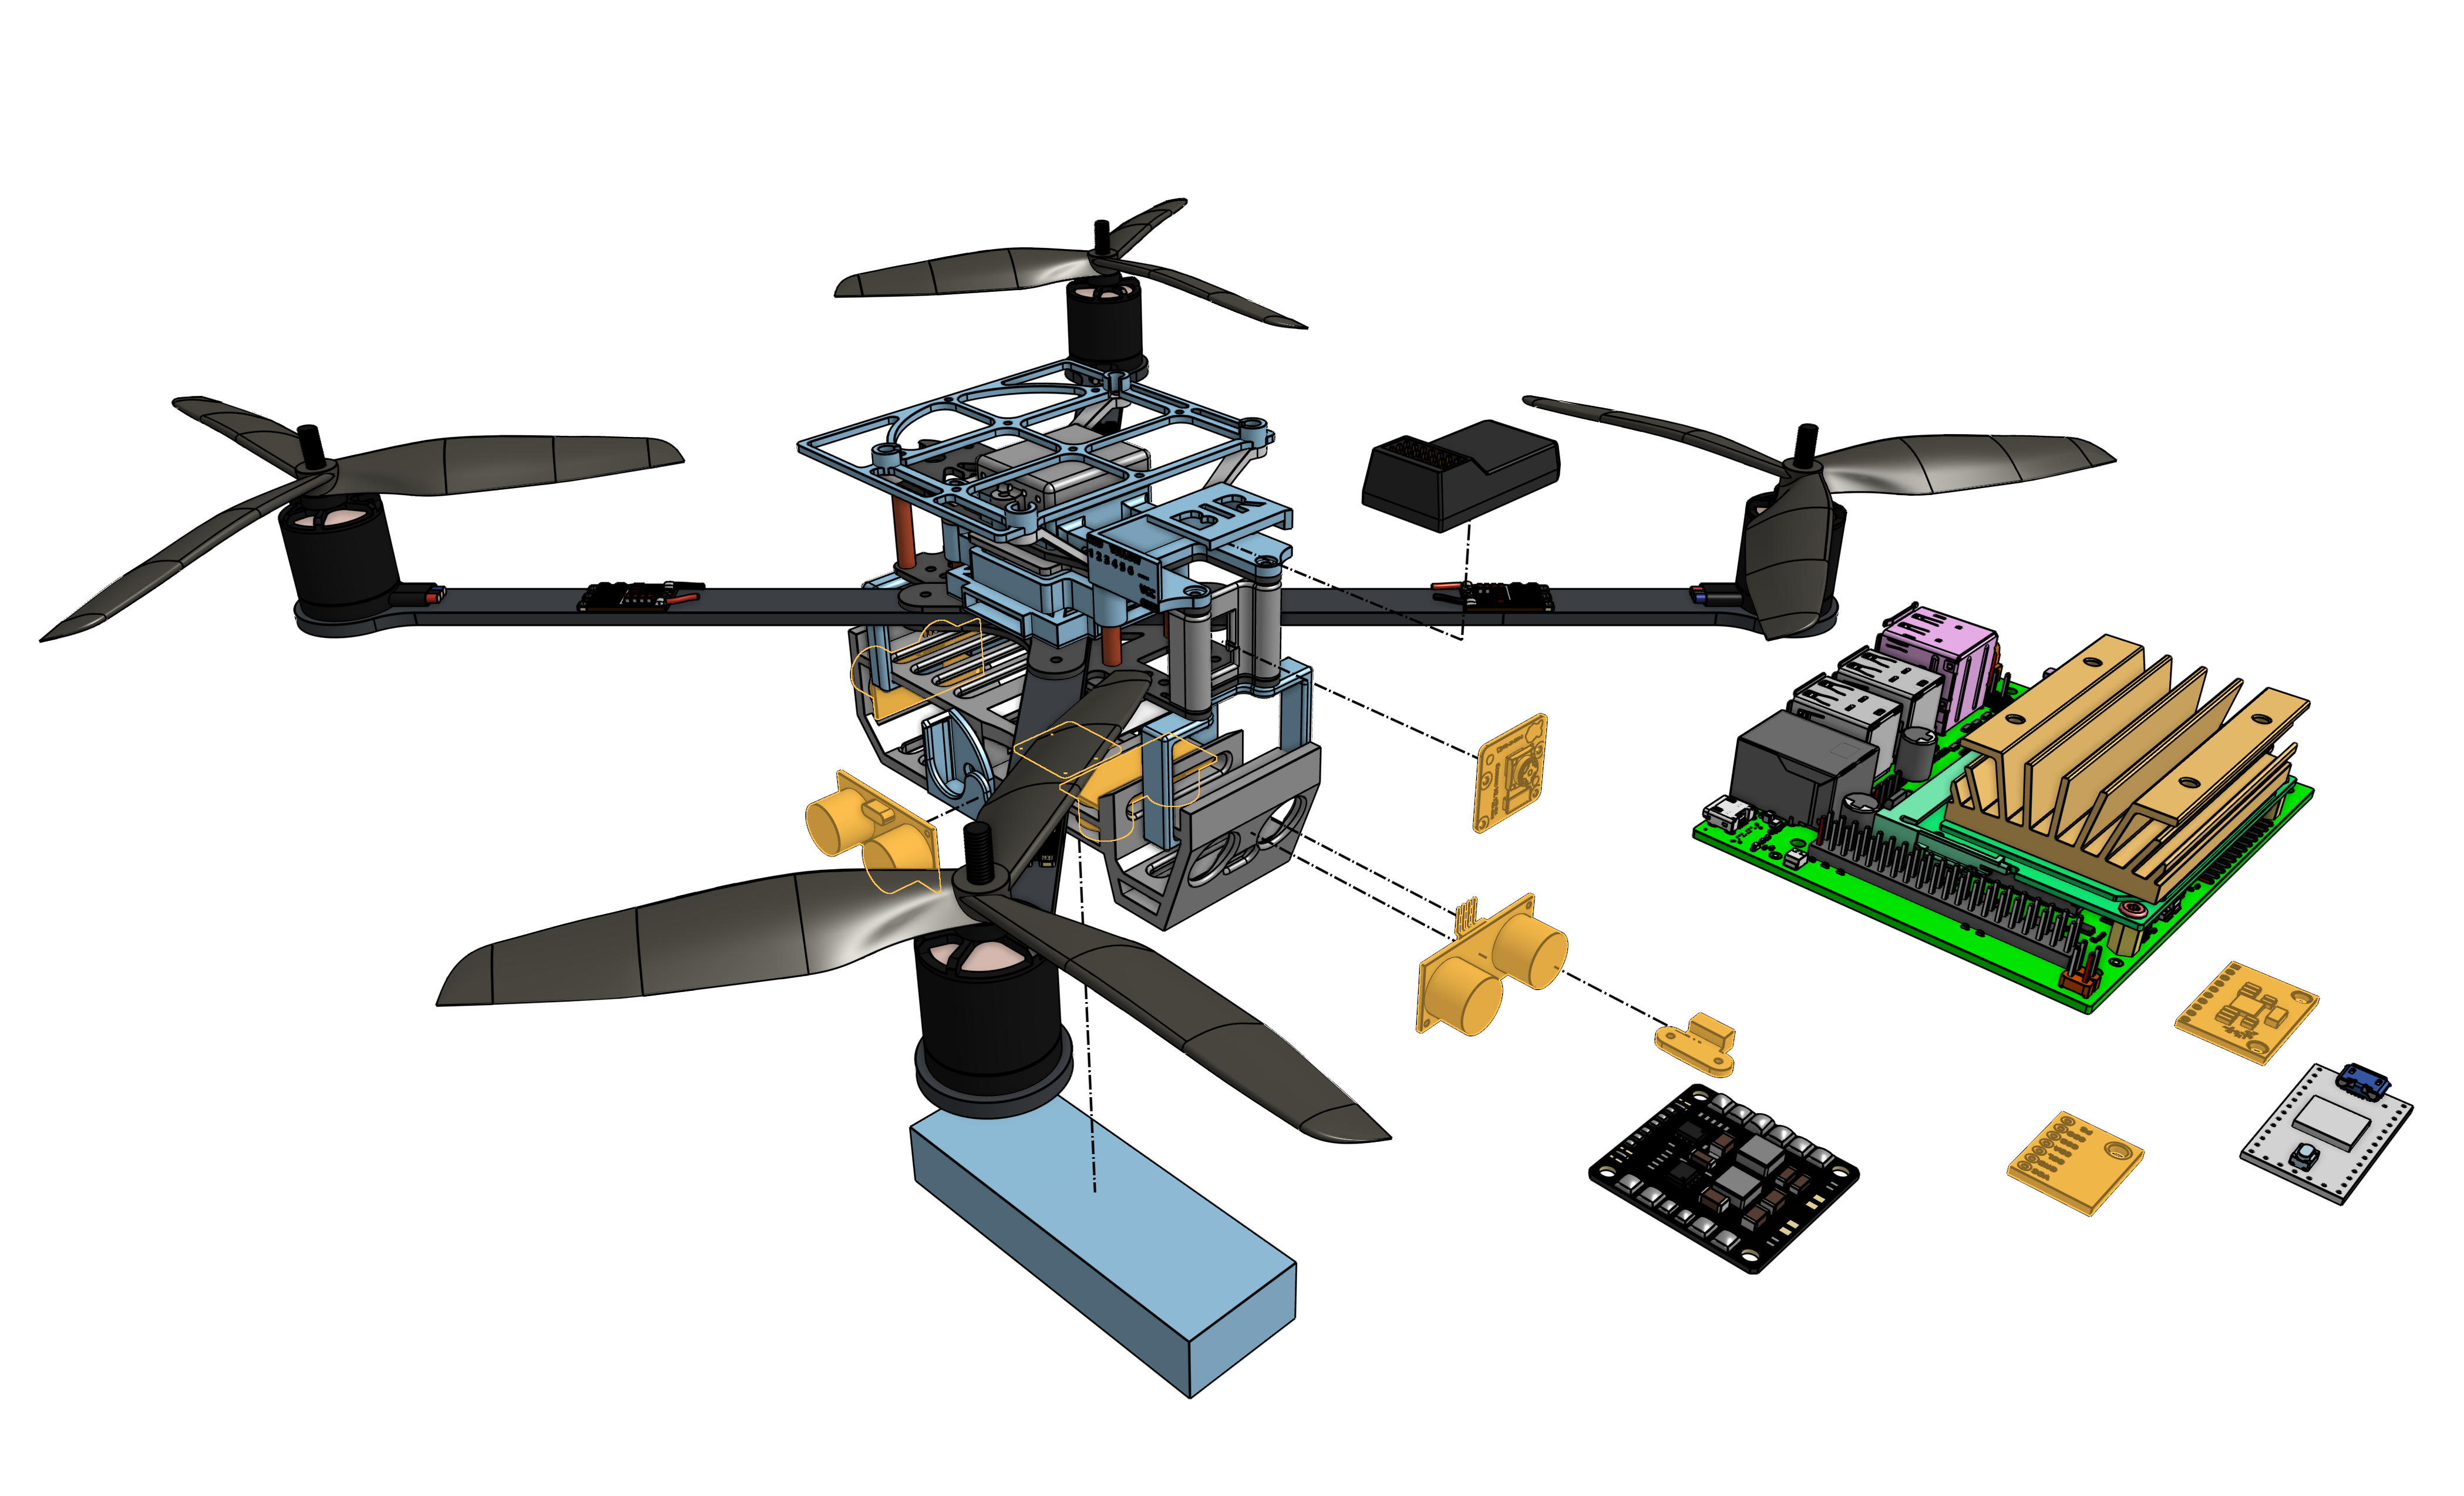
\includegraphics[width=1\textwidth]{img/exploded-sensors.png}
                \label{fig:sensors}
            \end{figure}
        \end{column}
    \end{columns}
\end{frame}

\begin{frame}{System Specification - Processing Power}


    \begin{columns}
        \begin{column}{0.4\textwidth}
        \begin{itemize}
            \item NVIDIA Jetson Nano Development Kit
            \item Microcontroller Teensy 4.0
            % \item MPU-9250 IMU
            % \item Matek Mini Power Hub
            % \item Lipo Battery 5000mAh 60C 3S
            % \item 4 x ESC Racestar 30A
            % \item 4 x Brushless Motor X2212 - 13 KV 980 II
        \end{itemize}
        \end{column}
        \begin{column}{0.6\textwidth}  %%<--- here
            \begin{figure}
                \centering
                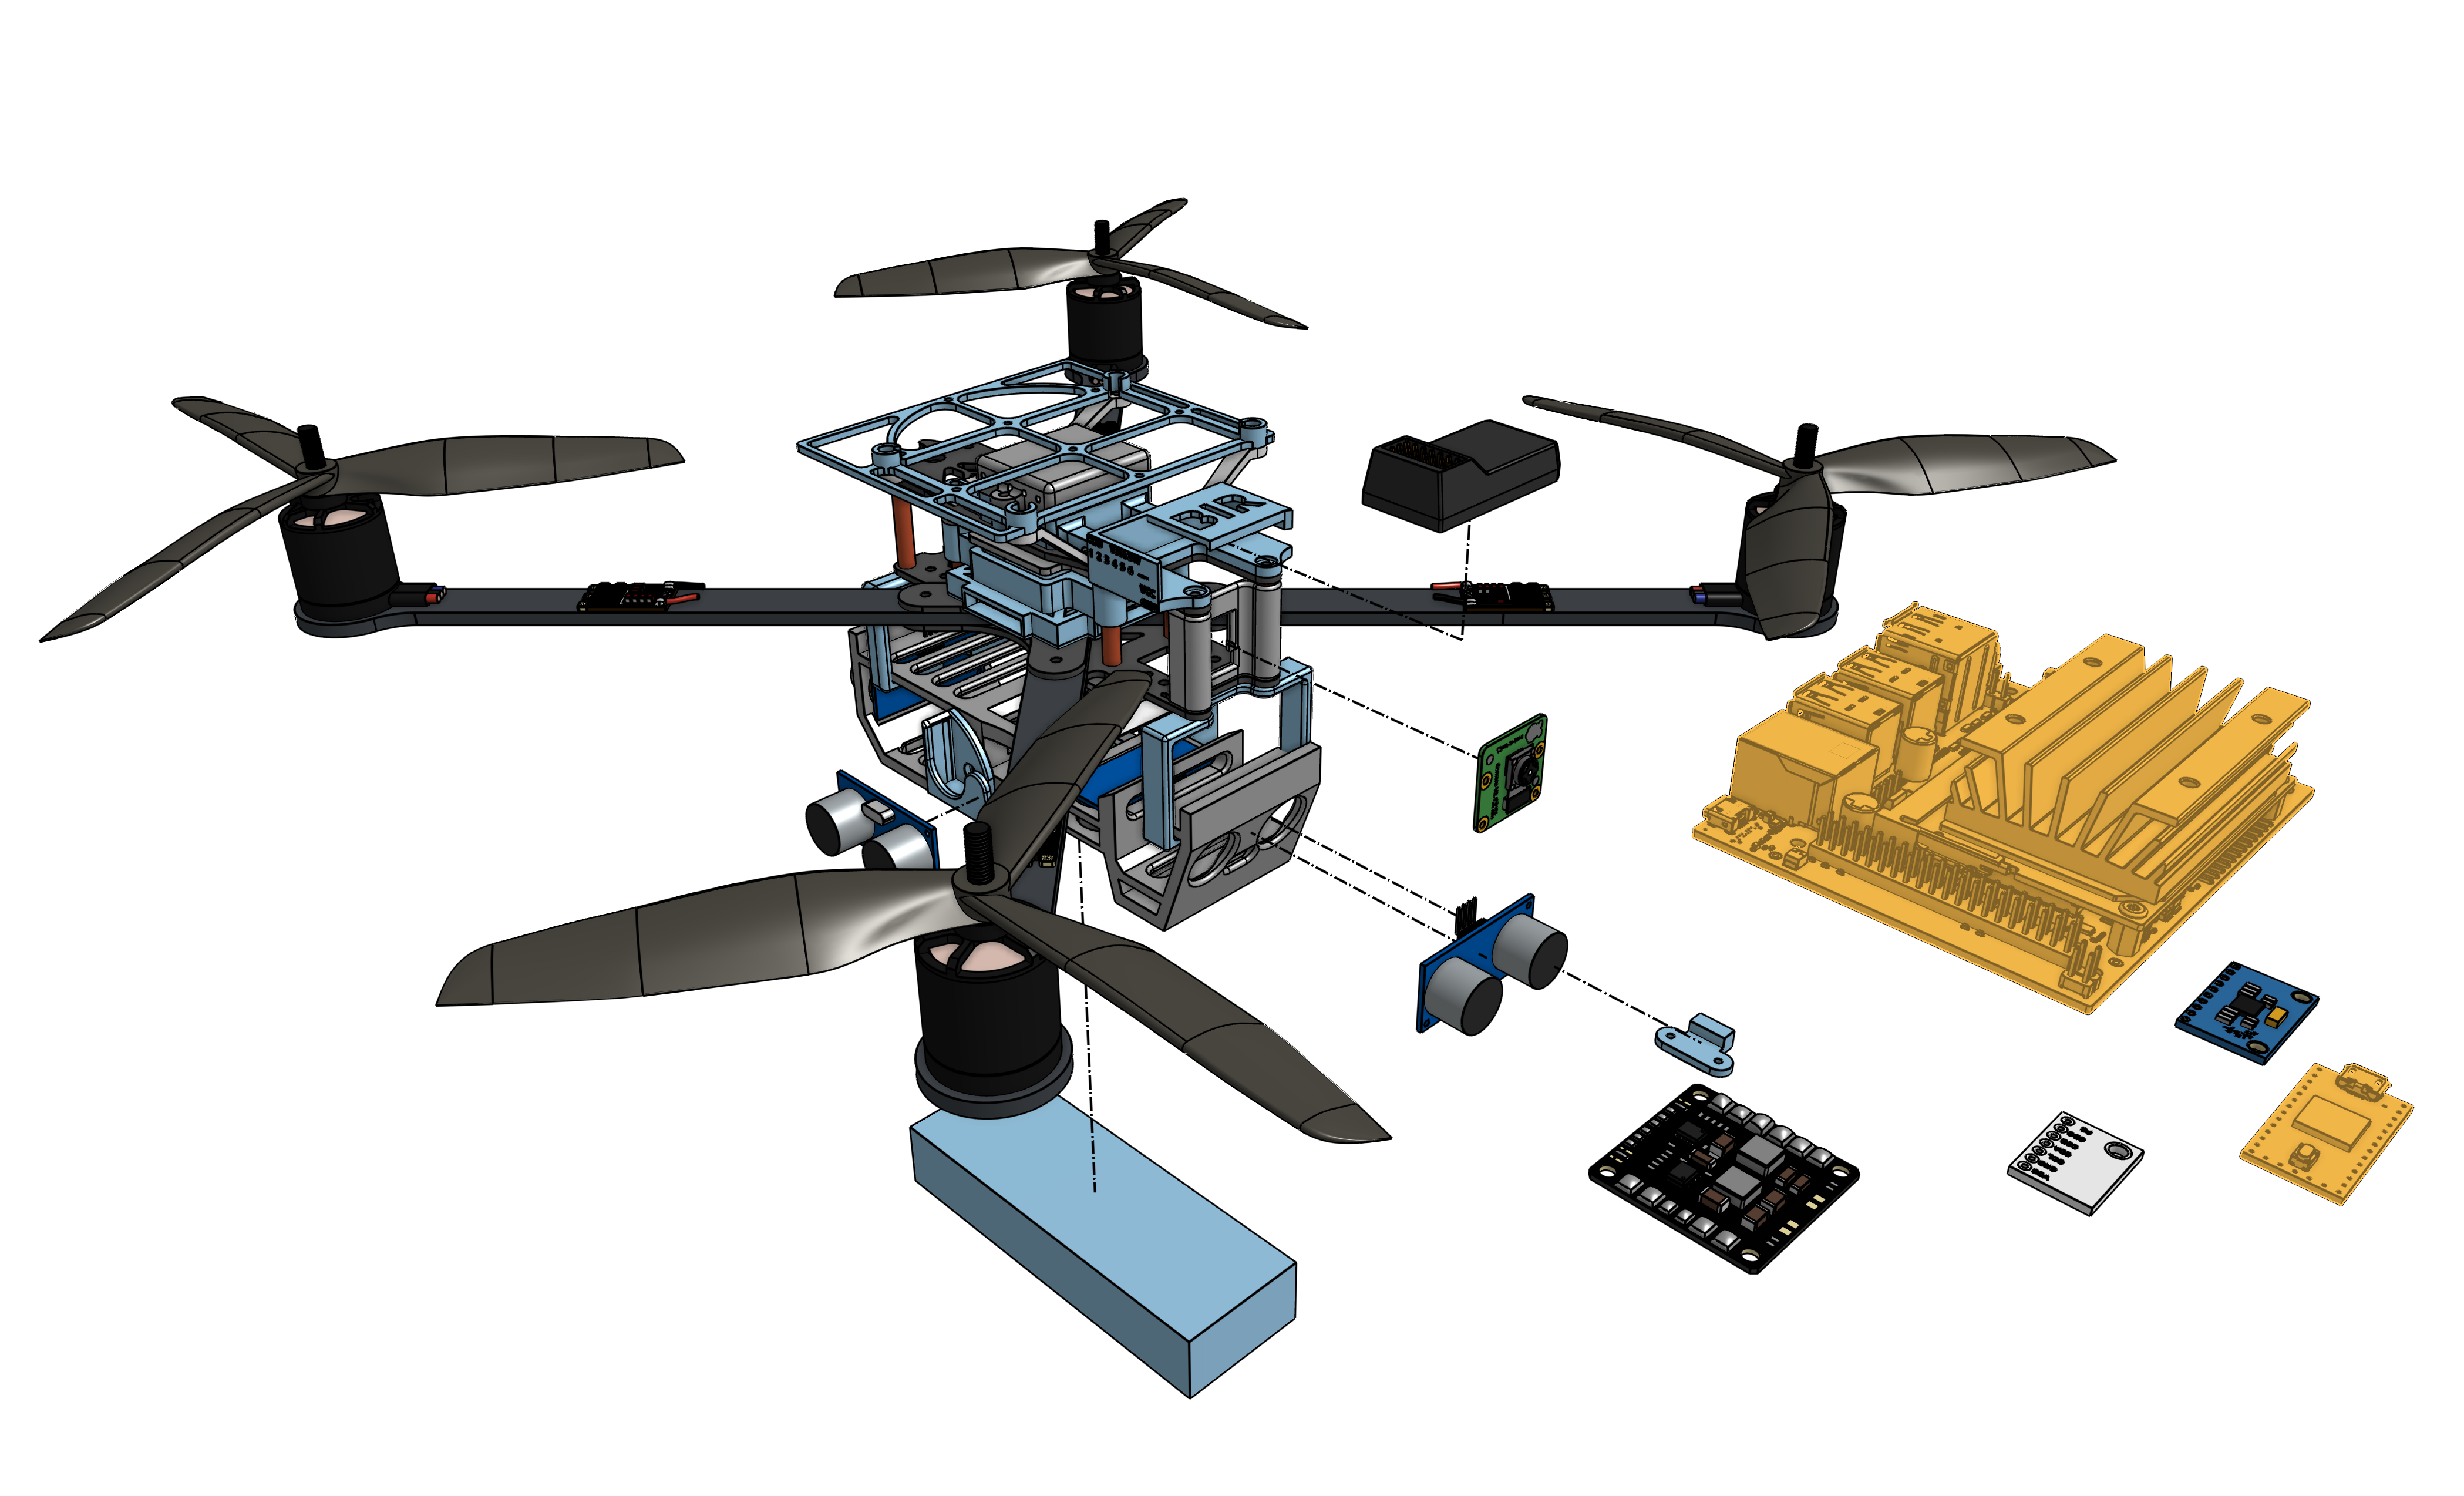
\includegraphics[width=1\textwidth]{img/exploded-processing.png}
                \label{fig:processing}
            \end{figure}
        \end{column}
    \end{columns}
\end{frame}

\begin{frame}{System Specification - Communication}


    \begin{columns}
        \begin{column}{0.4\textwidth}
        \begin{itemize}
            % \item NVIDIA Jetson Nano Development Kit
            % \item Microcontroller Teensy 4.0
            % \item MPU-9250 IMU
            % \item Matek Mini Power Hub
            % \item Lipo Battery 5000mAh 60C 3S
            % \item 4 x ESC Racestar 30A
            % \item 4 x Brushless Motor X2212 - 13 KV 980 II
            \item Radio Receiver (FS-R6B)
            \item Wifi Adapter (AC600)
        \end{itemize}
        \end{column}
        \begin{column}{0.6\textwidth}  %%<--- here
            \begin{figure}
                \centering
                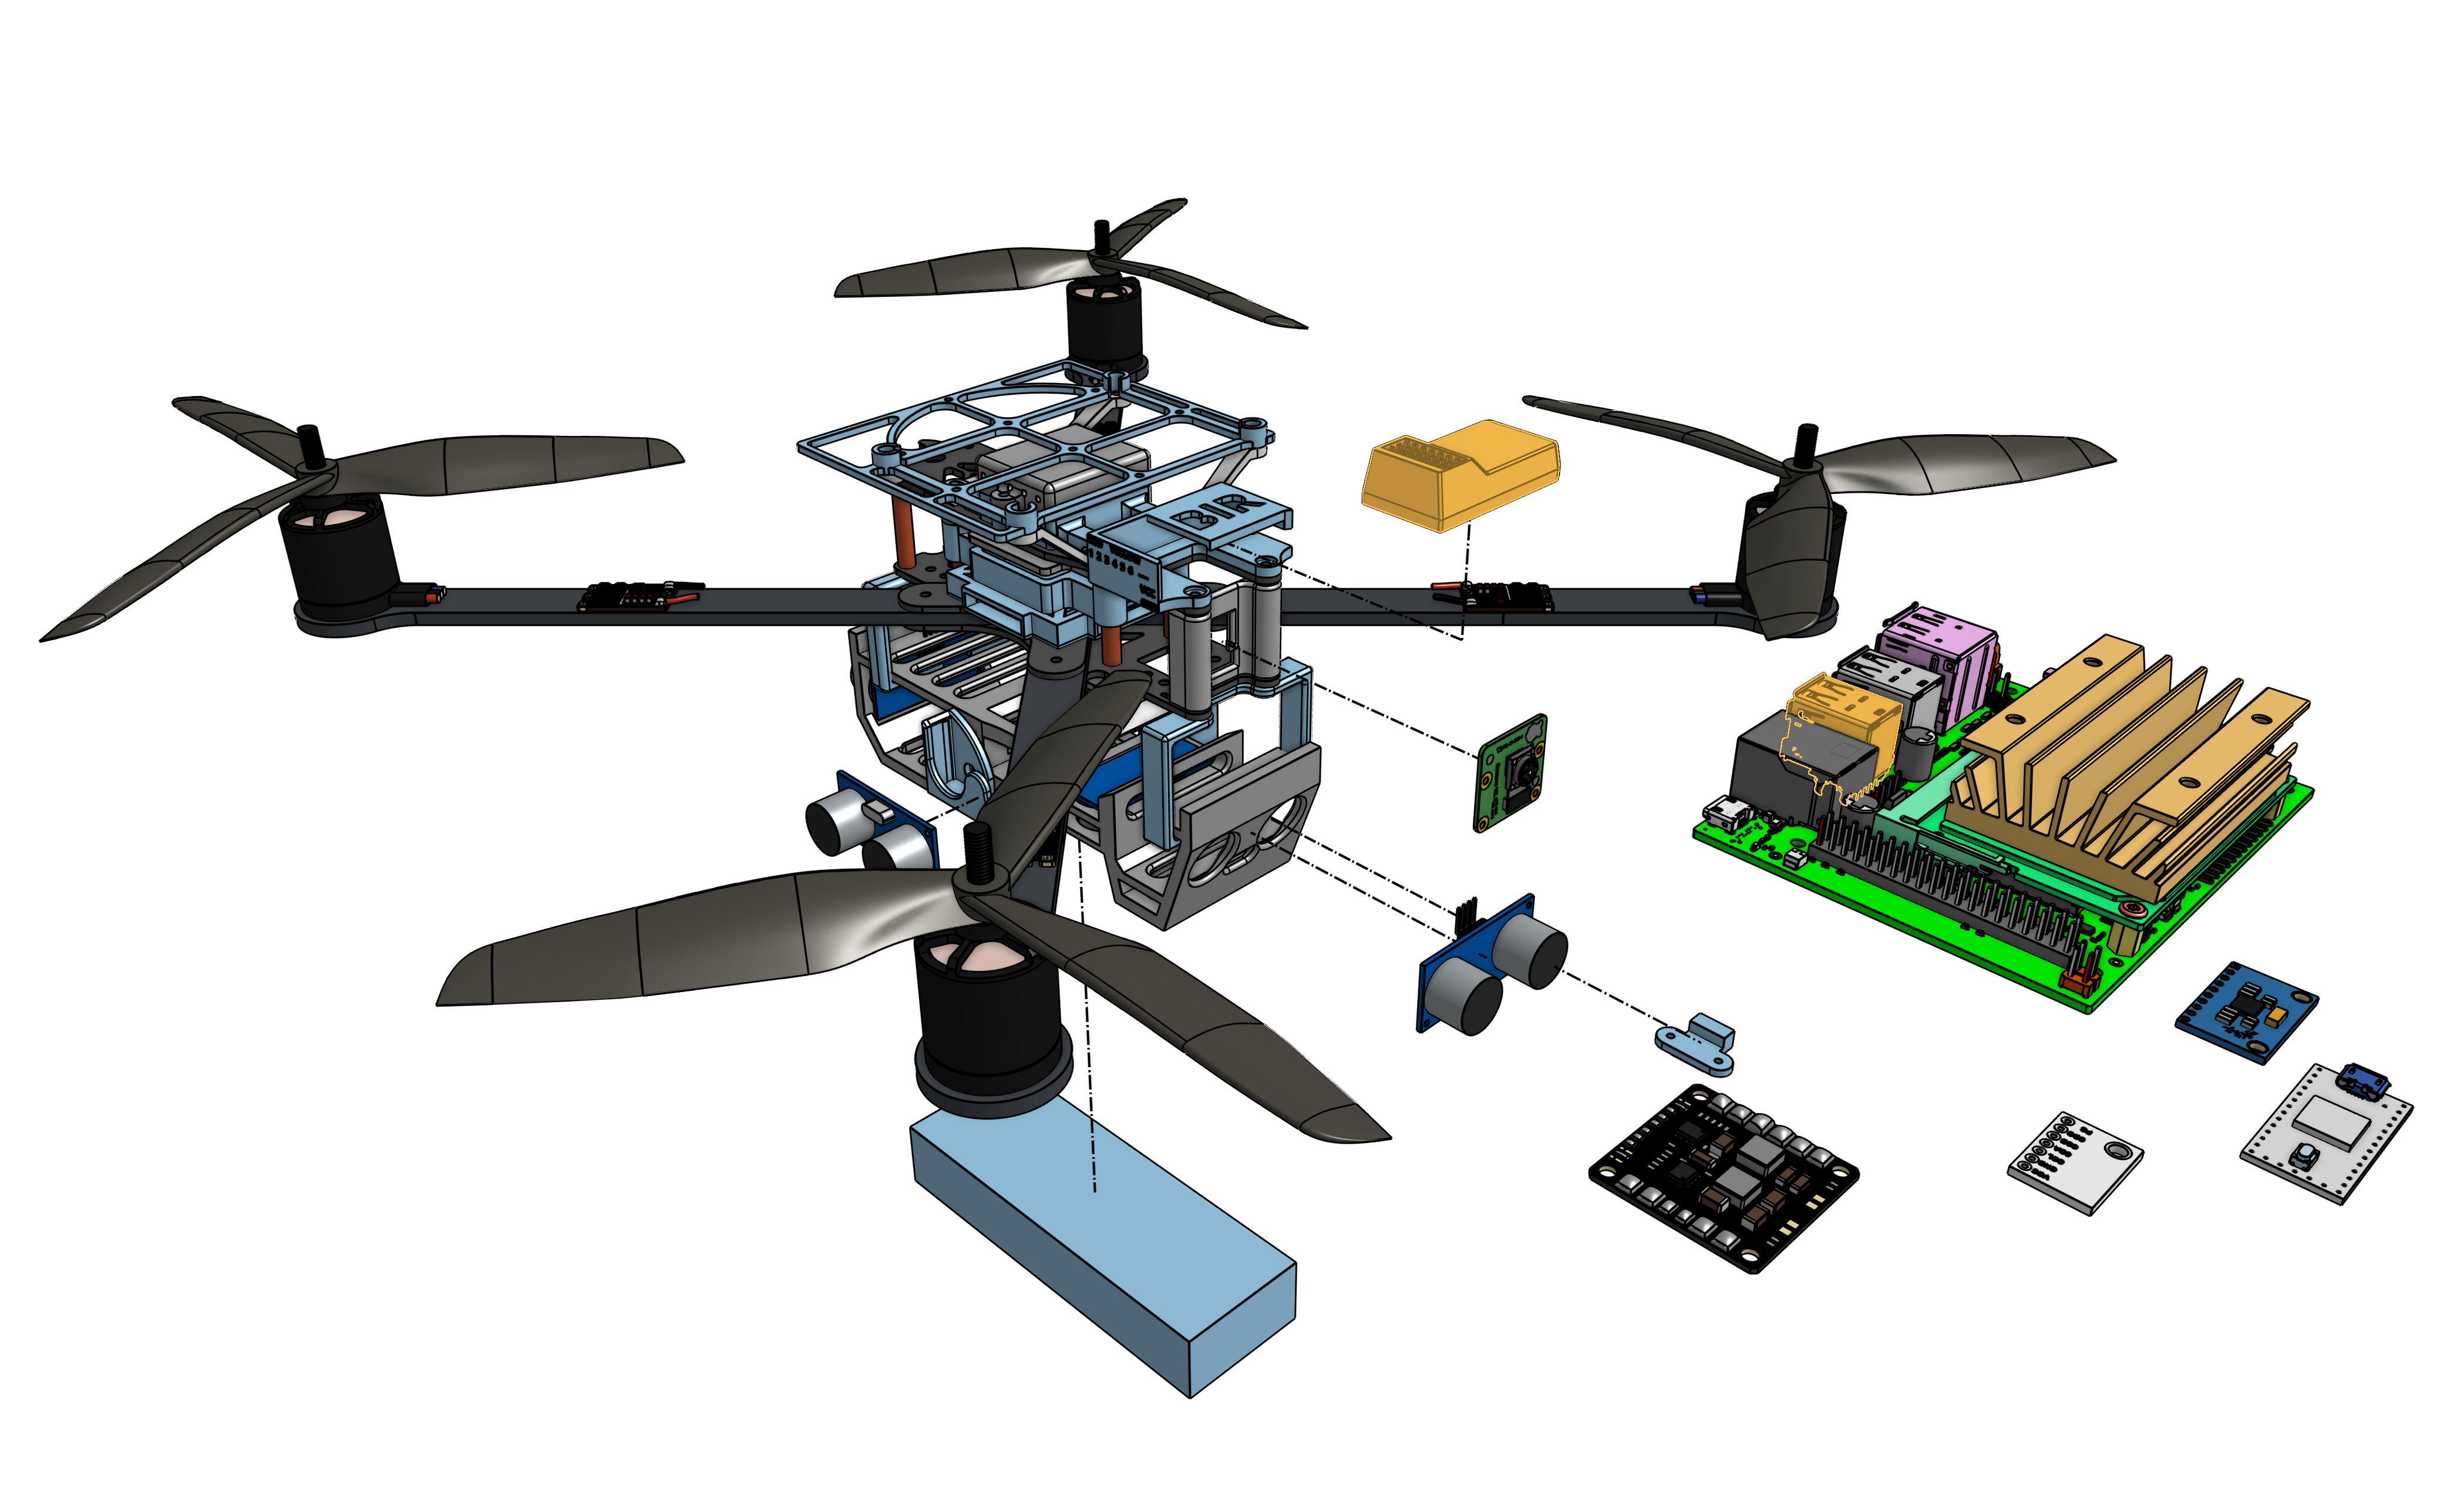
\includegraphics[width=1\textwidth]{img/exploded-comms.png}
                \label{fig:comms}
            \end{figure}
        \end{column}
    \end{columns}
\end{frame}

\begin{frame}{Electrical Schematic}
            \begin{figure}
                \centering
                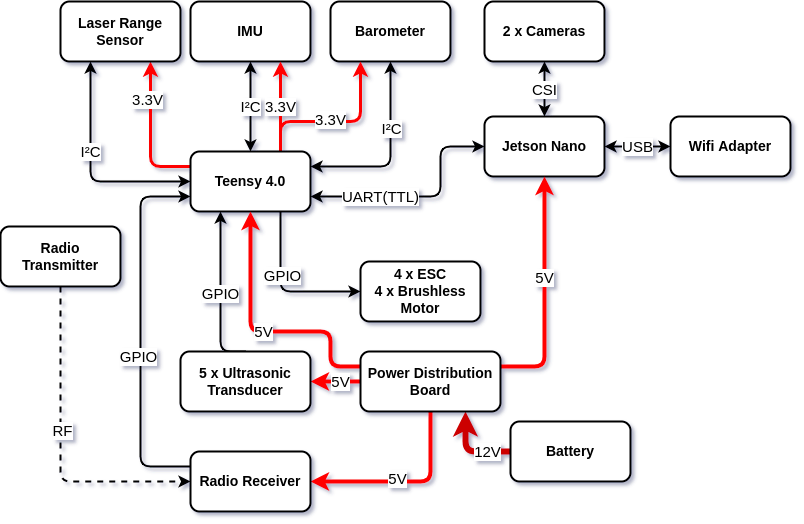
\includegraphics[width=0.6\textwidth]{img/esquematico.png}
                \label{fig:esquematico}
            \end{figure}

\end{frame}


\begin{frame}{Control Strategy}
    \begin{figure}
        \centering
        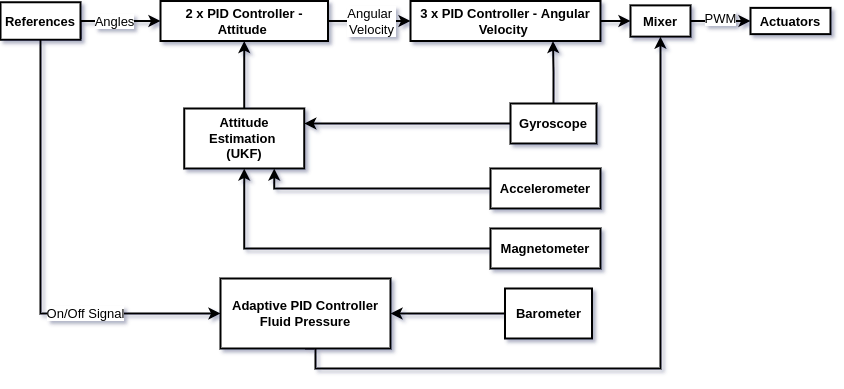
\includegraphics[width=0.8\textwidth]{img/control.png}
        \label{fig:esquematico}
    \end{figure}

\end{frame}


\begin{frame}{General Architecture}

\end{frame}

\begin{frame}{Results - Visualization}
        % \centering
        % \includemedia[
        %     width=0.8\linewidth,
        %     totalheight=0.45\linewidth,
        %     activate=pageopen,
        %     passcontext,
        %     addresource=./video/rviz_edit.mp4,
        %     flashvars={
        %     source=./video/rviz_edit.mp4
        %     &autoPlay=true
        %     &Loop=false}
        %     ]{\fbox{}}{VPlayer.swf}

\end{frame}

\begin{frame}{Results - Visualization}
        % \centering
        % \includemedia[
        %     width=0.8\linewidth,
        %     totalheight=0.45\linewidth,
        %     activate=pageopen,
        %     passcontext,
        %     addresource=./video/rosboard_edit.mp4,
        %     flashvars={
        %     source=./video/rosboard_edit.mp4
        %     &autoPlay=true
        %     &Loop=false}
        %     ]{\fbox{}}{VPlayer.swf}

\end{frame}

\begin{frame}{Results - Visualization}
        % \centering
        % \includemedia[
        %     width=0.8\linewidth,
        %     totalheight=0.45\linewidth,
        %     activate=pageopen,
        %     passcontext,
        %     addresource=./video/rosboard_edit2.mp4,
        %     flashvars={
        %     source=./video/rosboard_edit2.mp4
        %     &autoPlay=true
        %     &Loop=false}
        %     ]{\fbox{}}{VPlayer.swf}

\end{frame}

\begin{frame}{Results - Object Detection}
        % \centering
        % \includemedia[
        %     width=0.8\linewidth,
        %     totalheight=0.45\linewidth,
        %     activate=pageopen,
        %     passcontext,
        %     addresource=./video/objectdetection1_edit.mp4,
        %     flashvars={
        %     source=./video/objectdetection1_edit.mp4
        %     &autoPlay=true
        %     &Loop=false}
        %     ]{\fbox{}}{VPlayer.swf}
\end{frame}

\begin{frame}{Results - Pose Estimation}
        % \centering
        % \includemedia[
        %     width=0.8\linewidth,
        %     totalheight=0.45\linewidth,
        %     activate=pageopen,
        %     passcontext,
        %     addresource=./video/posenet2_edit.mp4,
        %     flashvars={
        %     source=./video/posenet2_edit.mp4
        %     &autoPlay=true
        %     &Loop=false}
        %     ]{\fbox{}}{VPlayer.swf}
\end{frame}

\begin{frame}{Results - ORB\_SLAM2}
        % \centering
        % \includemedia[
        %     width=0.8\linewidth,
        %     totalheight=0.45\linewidth,
        %     activate=pageopen,
        %     passcontext,
        %     addresource=./video/ORB_SLAM2_edit.mp4,
        %     flashvars={
        %     source=./video/ORB_SLAM2_edit.mp4
        %     &autoPlay=true
        %     &Loop=false}
        %     ]{\fbox{}}{VPlayer.swf}

\end{frame}


\begin{frame}{Results - Free Flight}
        % \centering
        % \includemedia[
        %     width=0.8\linewidth,
        %     totalheight=0.45\linewidth,
        %     activate=pageopen,
        %     passcontext,
        %     addresource=./video/height_control_edit.mp4,
        %     flashvars={
        %     source=./video/height_control_edit.mp4
        %     &autoPlay=true
        %     &Loop=false}
        %     ]{\fbox{}}{VPlayer.swf}
\end{frame}

\begin{frame}{Results - Pusher Configuration (Extra)}
        \begin{columns}
                \begin{column}{0.5\textwidth}
                        \begin{figure}
                                \centering
                                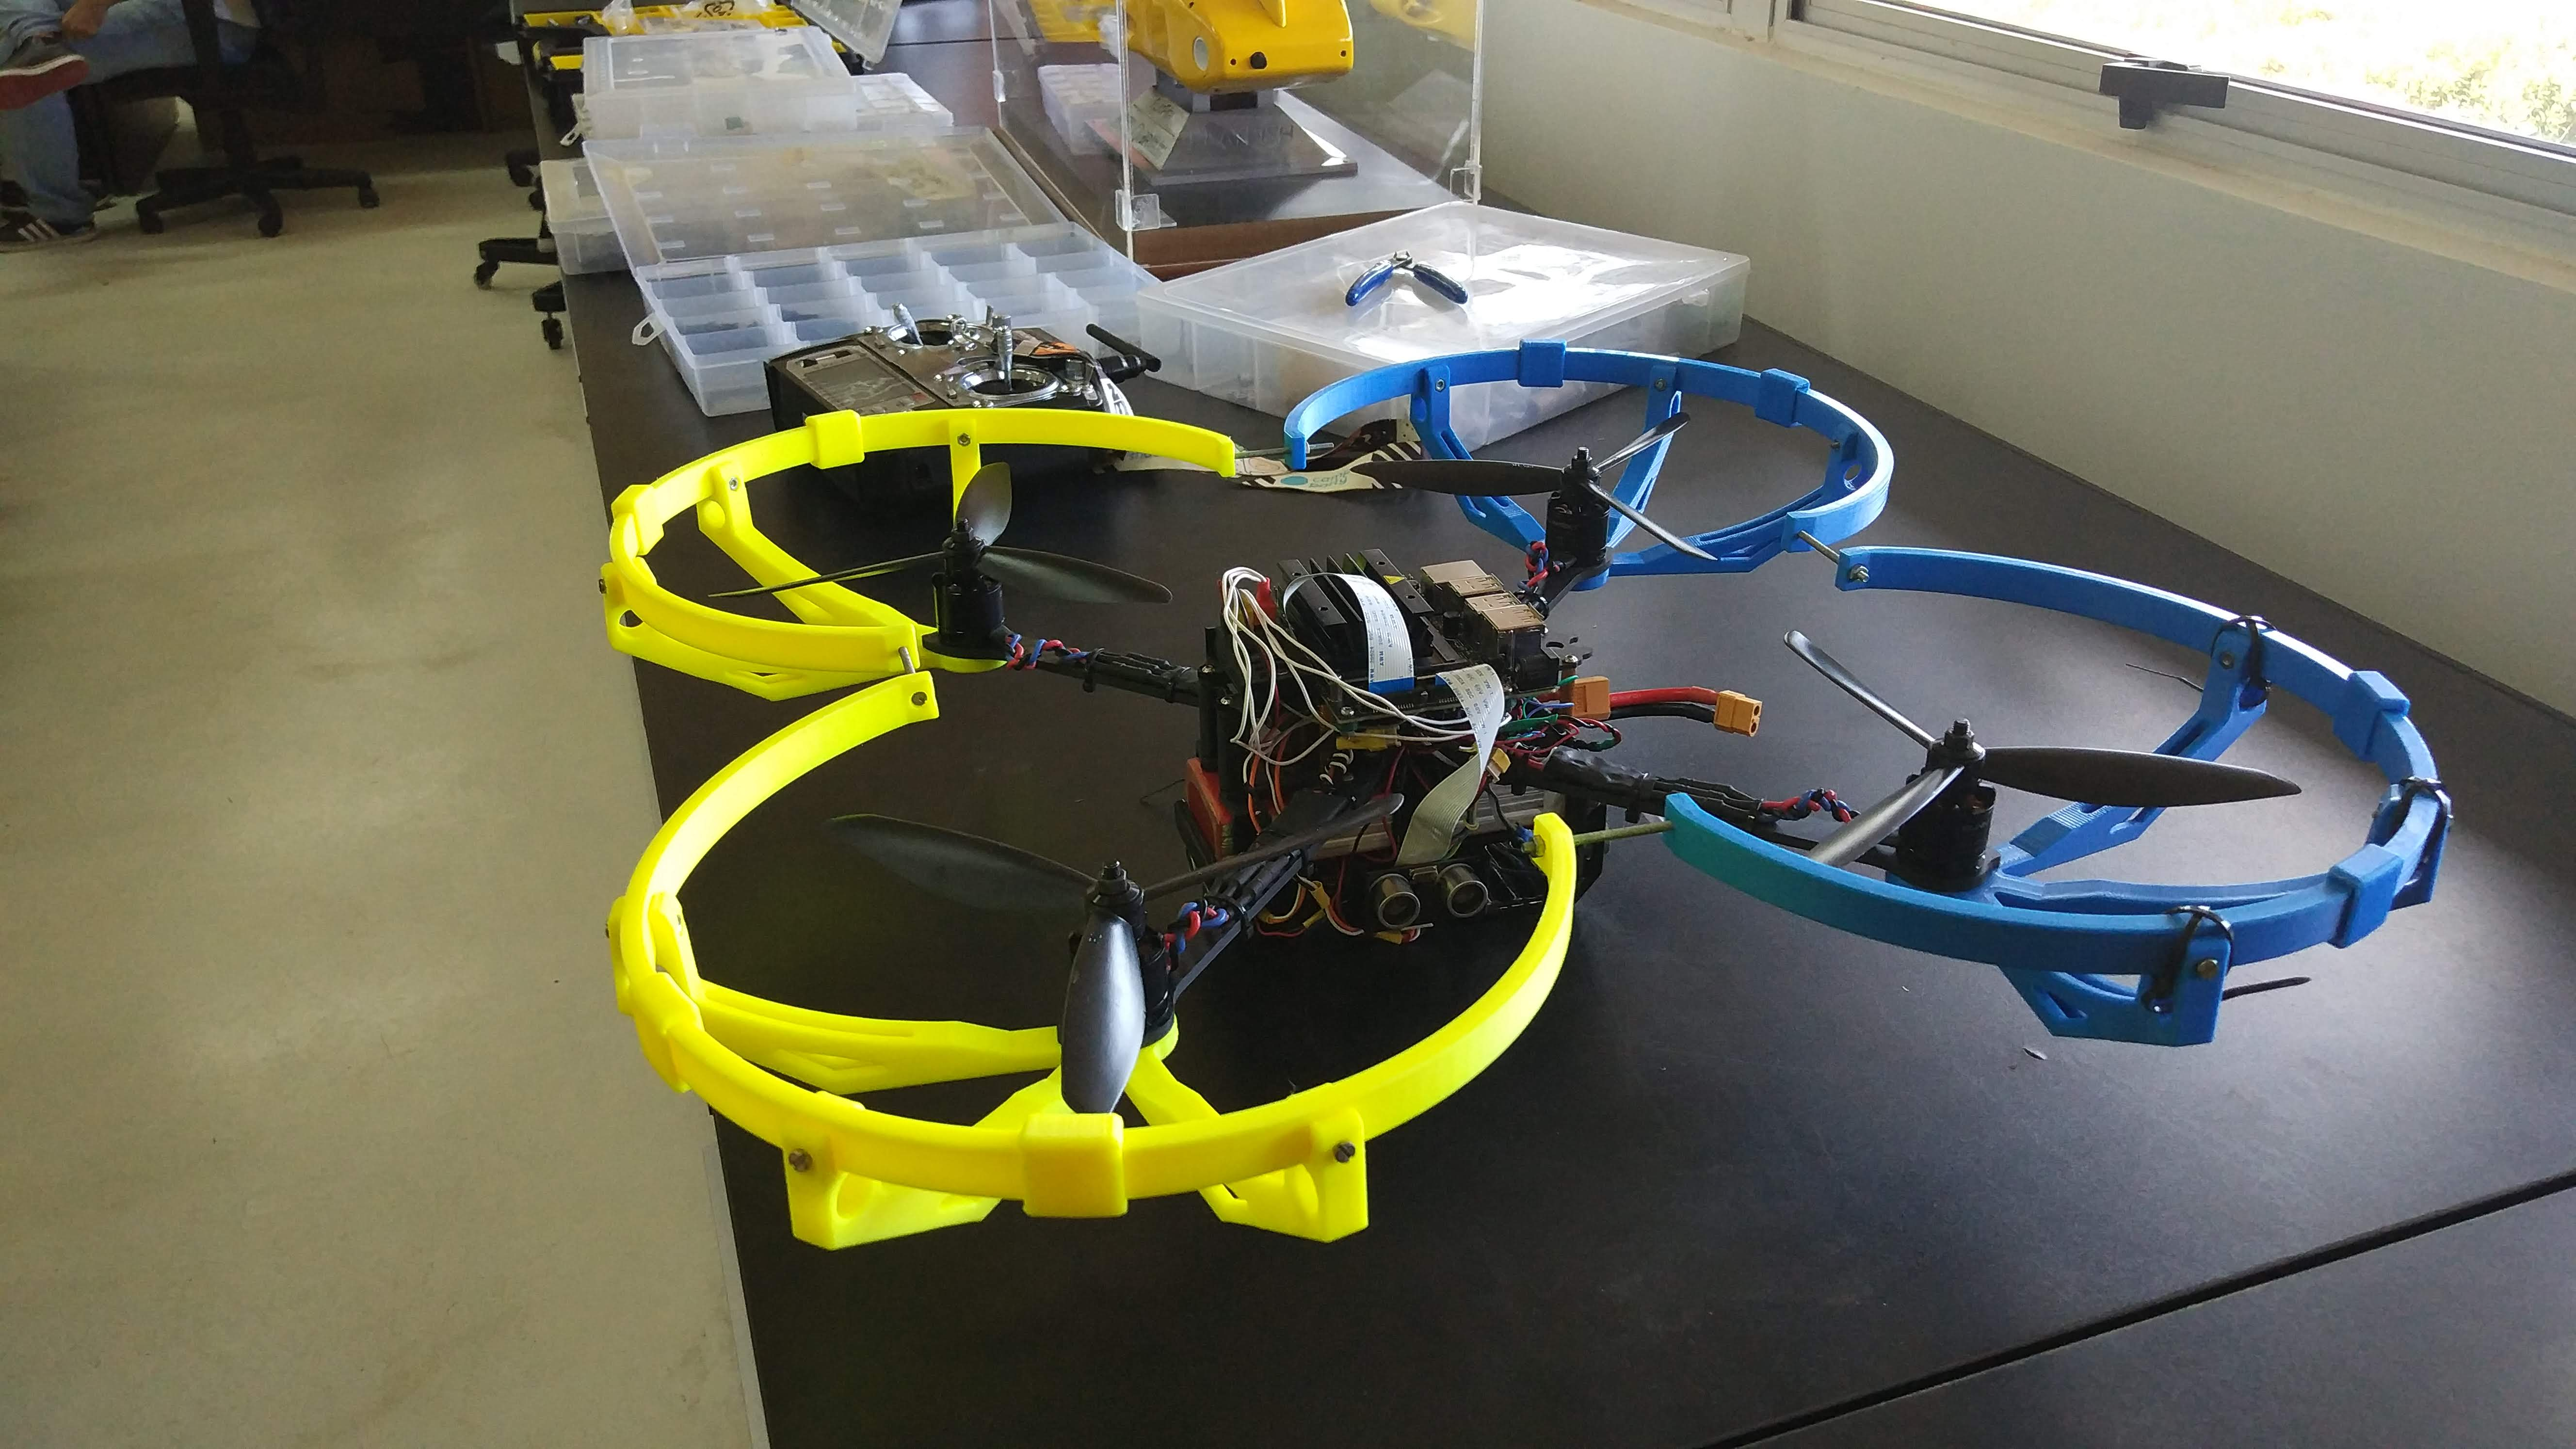
\includegraphics[width=1\textwidth]{img/protection.jpg}
                                \label{fig:prot}
                            \end{figure}
                \end{column}
                \begin{column}{0.5\textwidth}  %%<--- here

                %     \centering
                %     \includemedia[
                %         width=1\linewidth,
                %         totalheight=0.58\linewidth,
                %         activate=pageopen,
                %         passcontext,
                %         addresource=./video/bancada.mp4,
                %         flashvars={
                %         source=./video/bancada.mp4
                %         &autoPlay=true
                %         &Loop=false}
                %         ]{\fbox{}}{VPlayer.swf}
                \end{column}
            \end{columns}
\end{frame}


% %----------------------------------------------------SLIDE------------------
 \begin{frame}[t, allowframebreaks]{References}
 %\frametitle{References}
%\begin{frame}{Reference}
    %\transboxin[duration=1,direction=30]

    % \begin{bibunit}[plain]
    % \cite{guangyi2018research}.
    % %\cite{kanakia2012}
    % %\cite{agostini2007}
    % %\cite{azuma1997survey}
    % \cite{Buss2005}
  
    % \putbib
    % \end{bibunit}
  
    %\bibliographystyle{IEEEtran}
    %\bibliographystyle{IEEEtranS}
    %\bibliographystyle{IEEEbib}
    \bibliographystyle{abntex2-alf}
    %\bibliographystyle{abntex2-num}
    %\bibliographystyle{abnt-alf}
    \bibliography{bibliography} 
    %\putbib

%*----------- notes
    %\note[item]{Notes can help you to remember important information. Turn on the notes option.}
\end{frame}
%
%-
%*----------- SLIDE-BACKUP ------------------------------------------------------
% \backupbegin
% %
% \begin{frame}{Backup}
%     Test
% %*----------- notes-------------------------------
% \note{Notes can help you to remember important information. Turn on the notes option.}
% \end{frame}
% %-
% \backupend
% %-
%*----------- QUESTIONS ---------------------------------------------------------
\begin{frame}[c,plain]
    \lastpage{
        \begin{center}
            {\usebeamerfont{title} Questions?}\\[3ex]
            %\hspace{1.5cm}
            diogomartins.ac@gmail.com
        \end{center}
    }

    %*----------- notes---------------------------------
    \note[item]{Notes can help you to remember important information. Turn on the notes option.}
\end{frame}
%*-------------------------------------------------------------------------------
\end{document}